\documentclass{uclamsc}

\includeonly{
      capitulos/cv-tutor,
      capitulos/introduccion, 
      capitulos/el-problema, 
      capitulos/marco-teorico, 
      capitulos/marco-metodologico, 
	  capitulos/aspectos-administrativos,
}

% \habilitarpendientes	
% \habilitarnotas

\bibliografia{trabajo}

% Sobre el autor
\autor{Germán A. Gómez}
\citarcomo{Gómez}

% Sobre el trabajo
\titulo{ALGORITMO BASADO EN LÓGICA DIFUSA PARA SELECCIONAR  PROYECTOS DE APLICACIONES MÓVILES UTILIZANDO CRITERIOS IMPRECISOS}
% \title{mi trabajo}
\palabrasclave{algoritmo, lógica difusa, selección de proyectos, aplicaciones móviles, criterios imprecisos, conjuntos difusos.}% \keywords{}
\grado{Magister Scientiarum}

% Sobre la universidad
\decanato{DE CIENCIAS Y TECNOLOGÍA}
\postgrado{MAESTRÍA EN CIENCIAS DE LA COMPUTACIÓN MENCIÓN INTELIGENCIA ARTIFICIAL}
	
% Sobre el tutor
\tutor{Msc. Carlos I. Lameda Montero}

% Sobre la defensa
\ciudad{Barquisimeto}
% \diadefensa{}
% \mesdefensa{}
% \monthdefensa{}
\annodefensa{Mayo 2016}
% \primerjurado{}
% \segundojurado{}	

% Opcionales
% \mesencaratula
% \fechaenresumen

\begin{document}
	% Si se va a usar el glosario
	% %!TEX root = ../trabajo.tex 
	
	\resumen{%!TEX root = ../trabajo.tex
El significativo crecimiento del mercado de tecnologías móviles y la alta competitividad en el desarrollo de sus aplicaciones hace imperioso optimizar el uso de los recursos de una organización ---tiempo, dinero y esfuerzo---, necesarios en el inicio del desarrollo de proyectos, por lo que la decisión de priorizar y evaluar proyectos es un punto álgido en toda organización. El presente trabajo de investigación tiene como objetivo diseñar un algoritmo para sistemas de soporte de decisiones, que permita a los usuarios hacer elecciones con base en criterios subjetivos e imprecisos que serán representados mediante conjuntos difusos,  siendo más acordes a la naturaleza de los proyectos de aplicaciones móviles, al tratarse del desarrollo de nuevos productos. Esta investigación se hará bajo la modalidad de estudios de proyectos, fundamentada en investigación monográfica documental. Cabe resaltar que el presente trabajo estará orientado desde la perspectiva de la investigación tecnológica con un enfoque en la ciencia del diseño. En la propuesta se identificarán los criterios representativos y las tareas necesarias para la evaluación de proyectos de aplicaciones móviles, seguido del desarrollo de las etapas de análisis y conformación del algoritmo para la toma de decisiones en base a los criterios anteriormente definidos y finalmente se evaluará el algoritmo propuesto.}	
	\abstract{%!TEX root = ../trabajo.tex

}	

\begin{preliminares}
	\hacercaratula
	\hacerpresentacion
	\hacerindices
	%!TEX root = ../trabajo.tex
	\begin{tabular}{ c  p{11cm} }
    		\raisebox{-\totalheight}{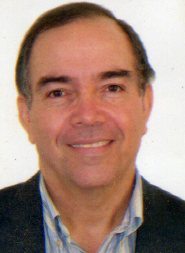
\includegraphics[width=0.15\textwidth]{graficas/CarlosL.jpg}}
    		& 
     	\begin{itemize}[topsep=0.1pt]
     }
     	\item[] 	\begin{Large}
     	\textbf{CARLOS  LAMEDA MONTERO}
     	\end{Large}
     	\item[] \textbf{RESUMEN CURRICULUM VITAE}
     	\end{itemize}	
     \end{tabular}

\begin{footnotesize}

   	\begin{itemize}
   	\item Ingeniero Electrónico, Instituto Universitario Politécnico de Barquisimeto, Venezuela, 1975.
    \item Master of Science en Ingeniería Eléctrica, Universidad de Stanford, USA, 1979.
 	\item Diploma de Estudios Avanzados en el área de Ingeniería de Sistemas y Automática, UNED, España, 2002.
 	\item Maestría en Ciencias de la Computación, Mención Inteligencia Artificial, UCLA, Venezuela, 2003.
	\item Estudios de Doctorado en Ciencias de la Ingeniería Mención Productividad, Universidad Nacional Experimental Politécnica Antonio José de Sucre (UNEXPO), escolaridad concluida en abril de 2015.
	\item Docente de la (UNEXPO), desde 1975 hasta el presente (2015).  Profesor Titular desde 1989.
	\item Jefe de la Sección de Control y Computación, Departamento de Ingeniería Electrónica, UNEXPO, 1980-87 y 1990-94.
	\item Director de Investigación y Postgrado, UNEXPO, Vicerrectorado Barquisimeto, 1995-1999.
Profesor jubilado de la UNEXPO desde marzo 2000.
	\item Coordinador de la Maestría en Ingeniería Electrónica de la UNEXPO (marzo 2003 – marzo 2007).
	\item De enero 2006 a abril 2016, Profesor de postgrado de las asignaturas Computación Emergente Aplicada a las Telecomunicaciones, Seminario de Investigación en Electrónica, Control Digital, Control Inteligente, Laboratorio de Simulación de Control Avanzado de Procesos, Control Adaptativo, Taller de Elaboración de Trabajo de Grado (UNEXPO), Lógica Difusa y Redes Neuronales, Modelos Lineales Aplicados a la Industria de Alimentos (UNELLEZ), Inteligencia Artificial, Sistemas Neurodifusos (Universidad de Carabobo), Sistemas Expertos (UCLA), Instrumentación Electrónica Avanzada (UNET).
   	\end{itemize}     
\newpage

\textbf{OTROS MÉRITOS Y ACTIVIDADES:}
 	\begin{itemize}
 	
 	\item Diseñador de la Opción Computación en Ingeniería Electrónica de la UNEXPO, 1982-1985.	
	\item Autor de 6 libros textos y guías de estudio de ingeniería.
	\item Autor de 36 trabajos de investigación.
	\item Coordinador de la Unidad de Proyectos Especiales (1996-1999), la cual ha recibido los premios  Innovación Tecnológica "Armada 97" (1997) y Excelencia Académica UNEXPO (1999). 
	\item Miembro de la Junta Administradora de la empresa pública ENELBAR (abril 2001- mayo 2003).
	\item Integrante de la Comisión Regional Centroccidental del Sistema para el Reconocimiento de Méritos a los Profesores de las Universidades Nacionales (2003). 
	\item Integrante de Comités Evaluadores de las Maestrías en Ingeniería Electrónica USB (2004) y UNET (2006), designado por el Consejo Nacional de Universidades (CNU). 
	\item “Technical Assistant” del equipo Waroz-UCLA, sub-campeón de la región Norte de Sur América ACM-ICPC World Internacional Programming Contest, participante en la final mundial, Tokio, Japón, abril 2007. 
	\item Conferencista en el VI Congreso Internacional de Electrónica y Tecnologías de Avanzada, Universidad de Pamplona, Colombia, marzo 2008. 
	\item Premios por trabajo de investigación y por trayectoria como investigador UNEXPO (1993), CONABA (1996), Orden "General Juan Jacinto Lara" 1ª Clase (1996), CONADES (1998), PPI (2005), PPI (2008), PEI (2011), PEI (2013), PEI (2015).
	\item Coordinador Iberoamericano de proyecto financiado por la Agencia Española de Cooperación Internacional para el Desarrollo (AECID) en colaboración con la UNED y la UNEXPO (2008-2009).
	\item Miembro de los Comités Organizadores de los Seminarios Nacionales sobre “Borrosidad y Sistemas Difusos”, “Inteligencia Artificial: Un Panorama de Aplicaciones” y “Modelos y Modelado” (2001-2015). 
    \item Conferencista en el I Congreso Internacional de Ingeniería de Sistemas en Inteligencia Computacional, Universidad Simón Bolívar sede Cúcuta, Colombia, septiembre 2015. 	
 	
 	\end{itemize}
\textbf{TRABAJOS DE GRADO DE MAESTRÍA TUTORADOS}

  \begin{flushleft}

\textbf{Año: 2016. Institución: Universidad Nacional Experimental Politécnica “Antonio José de Sucre” (UNEXPO)}\\
\begin{itemize}
\item “Sintonización de Controladores PID en Procesos de Primer y Segundo Orden Mediante Optimización por Enjambre de Partículas”\\
Nombre del estudiante: Henry Zapata\\ 
Título a Obtener: Magíster Scientiarum en Ingeniería de Control de Procesos    
\end{itemize}
  
\textbf{Año: 2014. Institución: Universidad Nacional Experimental Politécnica “Antonio José de Sucre” (UNEXPO)}\\
\begin{itemize}
\item “Control Difuso de la Velocidad Angular para una Turbina Eólica”\\
Nombre del estudiante: Manuel Díaz\\ 
Título a Obtener: Magíster Scientiarum en Ingeniería de Control de Procesos \\
\item “Control Adaptativo de Temperatura para un Reactor Continuo tipo Tanque Agitado”
Nombre del estudiante: Gerson Urbina 
Título a Obtener: Magíster Scientiarum en Ingeniería de Control de Procesos 
\end{itemize}

\textbf{Año: 2013. Institución: Universidad Nacional Experimental Politécnica “Antonio José de Sucre” (UNEXPO)}\\
\begin{itemize}
\item “Control de la Concentración de Etanol en el Tope de una Columna de Destilación Continua mediante un Sistema Adaptativo de Inferencia Neurodifusa”\\
Nombre del estudiante: Eumar Leal\\
Título a Obtener: Magíster Scientiarum en Ingeniería de Control de Procesos
\item “Control Robusto de la Concentración de Etanol en un Proceso de Cultivo Semicontinuo de Levaduras”\\
Nombre del estudiante: Antioquía Galicia\\
Título a Obtener: Magíster Scientiarum en Ingeniería de Control de Procesos 
\end{itemize}

\textbf{Año: 2013. Institución: Universidad Centroccidental Lisandro Alvarado (UCLA)}\\
\begin{itemize}
\item “Modelo Basado en Lógica Difusa para la Comparación de Objetos con Atributos Imprecisos”\\
Nombre del estudiante: Sheijer Silva\\
Título Obtenido: Magíster Scientiarum en Ciencias de la Computación.
\end{itemize}

\textbf{Año: 2011. Institución: Universidad Nacional Experimental Politécnica “Antonio José de Sucre” (UNEXPO)}\\
\begin{itemize}
\item “Software de Soporte para el Proceso de Enseñanza-Aprendizaje de un Laboratorio de Comunicaciones Digitales”\\
Nombre del estudiante: Celeste Leopardi\\
Título a Obtener: Magíster Scientiarum en Ingeniería Electrónica 
\item “Control Predictivo de Nivel de Agua y Presión de Vapor  para una Caldera”\\
Nombre del estudiante: Fermín García\\
Título a Obtener: Magíster Scientiarum en Ingeniería de Control de Procesos 
\end{itemize}


\textbf{Año: 2010. Institución: Universidad Nacional Experimental Politécnica “Antonio José de Sucre” (UNEXPO)}\\
\begin{itemize}
\item “Control Adaptativo de la Concentración de Etanol en un Proceso de Cultivo Semicontinuo de Levaduras”\\
Nombre del estudiante: Luz Marina Suárez\\
Título a Obtener: Magíster Scientiarum en Ingeniería de Control de Procesos
\item “Sistema de Control Difuso para la Alimentación de Sustrato en un Cultivo Semicontinuo de Levaduras”\\
Nombre del estudiante: Llelysmar Crespo\\
Título Obtenido: Magíster Scientiarum en Ingeniería de Control de Procesos 
\end{itemize}

\textbf{Año: 2009. Institución: Universidad Nacional Experimental Politécnica “Antonio José de Sucre” (UNEXPO)}\\
\begin{itemize}
\item “Control Difuso de Temperatura para un Horno a Gas”\\
Nombre del estudiante: Giovanny Rodríguez\\
Título Obtenido: Magíster Scientiarum en Ingeniería de Control de Procesos 
\item “Evaluación del Desempeño de Sistemas Neuro-Difusos en la Identificación de Canales de Radiocomunicaciones”\\ 
Nombre del estudiante: Ángel José León Peña\\
Título Obtenido: Magíster Scientiarum en Ingeniería Electrónica 
\end{itemize}

\textbf{Año: 2009. Institución: Universidad de Carabobo (UC). Título Obtenido: Magíster Scientiarum en Ingeniería Eléctrica}\\
\begin{itemize}

\item “Consultor Inteligente  para el Mantenimiento  de Redes LAN de Alta Velocidad Ethernet Basado en Agentes Inteligentes”\\
Nombre del estudiante: Marisela Materano
\item “Diseño de  un Sistema Experto para el Asesoramiento en las Operaciones de Mantenimiento de Redes WLAN Basado en Árboles de Decisión”\\
Nombre del estudiante: Yelmin Pérez
\end{itemize}
 
\textbf{Año: 2007. Institución: Universidad Centroccidental Lisandro Alvarado (UCLA)}\\
\begin{itemize}
\item “Sistema para la Determinación del Flujo en un Canal Vehicular Basado en Procesamiento de Imágenes y Redes Neuronales”\\  
Nombre del estudiante: Antonio Ferraz\\
Título Obtenido: Magíster Scientiarum en Ciencias de la Computación.
\end{itemize}

\textbf{Año: 2005. Institución: Universidad Centroccidental Lisandro Alvarado (UCLA)}\\
\begin{itemize}
\item “Sistema de Clasificación Neurodifusa en Imágenes de Envases”\\
Nombre del estudiante: Oscar Galindo\\
Título Obtenido: Magíster Scientiarum en Ciencias de la Computación.
\end{itemize}


\textbf{Año: 1997. Institución: Universidad Nacional Experimental Politécnica “Antonio José de Sucre” (UNEXPO)}\\
\begin{itemize}
\item “Diseño de un Controlador Digital Utilizando el Puerto Paralelo de un PC”\\
Nombre del estudiante: Carlos  Alberto Rey Soto\\
Título Obtenido: Magíster Scientiarum en Ingeniería Electrónica  
\end{itemize}

\textbf{Año: 1996.  Institución: UNEXPO}\\ 
\begin{itemize}
\item “Diseño y Construcción de un Electrocardiógrafo de un Canal Basado en Microcontroladores, Capaz de Funcionar como Sistema Remoto de Adquisición de Señal Eléctrica Cardíaca para un PC”\\ 
Nombre del estudiante: Humberto Barazarte\\
Título Obtenido: Magíster Scientiarum en Ingeniería Electrónica 
\item “Aplicación de Controladores Lógicos Programables “PLC”  en un Proceso Industrial de Trituración y Homogenización”\\ 
Nombre del estudiante: José Heliodoro Quintero\\
Título Obtenido: Magíster Scientiarum en Ingeniería Electrónica 
\item “Diseño e Implementación de un Sistema de Monitoreo por Computador de la Variables: Nivel, Temperatura y Flujo para una planta de Procesos Piloto”\\
Nombre del estudiante: Virgilio Baptista\\
Título Obtenido: Magíster Scientiarum en Ingeniería Electrónica 
\end{itemize}
 \end{flushleft}
\textbf{  ALGUNAS PUBLICACIONES}
\begin{flushleft}
\begin{itemize}
\item “ANFIS Neuro-Fuzzy modeling of a pneumatic leak testing system”. CDC-ECC 05, Sevilla, España. Diciembre 2005.
\item “La Inteligencia artificial y sus aportes a la física médica y la bioingeniería. En Publicaciones de la Comisión de Estudios Interdisciplinarios, UCV, Año 9, No 24, 2006, pp. 149-153.
\item “Clasificación de Lesiones Gástricas en Imágenes Endoscópicas mediante la Técnica de Pirámide Difusa  y Redes Neuronales”. CLAIB 2007. Venezuela, septiembre 2007.
\item “Herramienta computacional para la combinación balanceada de nutrientes utilizando lógica difusa y búsqueda heurística”, Revista de Ciencia y Tecnología Agrollanía, Volumen 5, 2008, pp. 1-10.
\item “Clasificador difuso neuronal aplicado a casos de enfermedades hepatobiliares representadas por datos con patrones solapados”,  Revista  Científica UNET, Volumen 20 Nº,1 2008, pp. 85-98.
\item “Extracción automática de características de vehículos en movimiento a partir de videos basada en red neuronal de Kohonen”.  Revista   Ingeniería UC, Volumen 15, N° 3, 2008, pp. 33-44.
\item “Design of a pH and temperature fuzzy control system for the production process of liquid ammonium nitrate”. 3rd Seminar for Advanced Industrial Control Applications. SAICA 2009. Madrid, España. 
\item “Sistema de control difuso para la alimentación de sustrato en un cultivo semicontinuo de levaduras”. XIV Congreso Latinoamericano de Control Automático, Santiago de Chile, agosto 2010.
\item “El Análisis Envolvente de Datos y el Índice de Malmquist como Técnicas Innovadoras en el Análisis de la Eficiencia y Productividad en Departamentos Académicos de Universidades Venezolanas”. Congreso Regional de Investigación y Pedagogía 2014. UPEL, Barquisimeto, Venezuela.
\item “Control para Alimentación de Sustrato en Cultivo De Lactococcus lactis”. 24º Congreso Argentino de Control Automático, 27 al 29 de Octubre de 2014 – Buenos Aires, Argentina.
\item “Métodos Relacionados con Diagnósticos de Fallas con Síntomas Imprecisos mediante Comparación ce Casos”. REDIP. Venezuela. Vol. 5. No. 3, 2015.
\item “Importancia de Publicar Artículos Científicos desde las Perspectivas Individual, de las Organizaciones y La Sociedad”. REDIP. Venezuela. Vol. 5. No. 4, 2015.

\end{itemize}
\end{flushleft}
\end{footnotesize}
	\hacerresumen
\end{preliminares}

\begin{contenido}
	%!TEX root = ../trabajo.tex
\introduccion
Se estima que el crecimiento del mercado global de aplicaciones móviles de los últimos tres años se encuentre cerca del 210\%, representando un crecimiento de \$143 mil millones en el año 2016,  Esto se debe principalmente al uso cotidiano de los dispositivos móviles, lo que ha conducido a demandas más altas en cuanto a la calidad y estabilidad de productos ofertados. Además, este significativo crecimiento ha dado lugar a un aumento en la importancia de una mejor interacción entre el usuario y la tecnología. Sin embargo, las tendencias móviles suelen cambiar rápido debido a su estrecha relación con el hardware, el cual se encuentra en una continua renovación y ocasiona que los productos duren un corto período de tiempo. Adicionalmente la alta competitividad en el desarrollo de aplicaciones hace imperioso optimizar el uso de los recursos de una organización -tiempo, dinero y esfuerzo-, necesarios en el inicio del desarrollo de proyectos, por lo que la decisión de priorizar y evaluar proyectos es un punto álgido en toda organización dedicada al desarrollo de software. Razón por la que se propone en el presente trabajo de investigación el diseño de un algoritmo para sistemas de soporte de decisiones, que permita a los usuarios hacer elecciones de  criterios de selección adecuados para los proyectos de aplicaciones móviles, mediante el uso de valoraciones subjetivas e imprecisas, representadas mediante conjuntos borrosos.\\

Este proyecto de investigación está estructurado en cuatro capítulos, conforme al manual para la elaboración del trabajo conducente a grado académico de especialización, maestría y doctorado de la UCLA (2002). En el primero, el planteamiento del problema, se exponen los diferentes elementos que conforman el entorno de la situación planteada con respecto a los criterios requeridos, así como también a los modelos de toma de decisiones que podrán contribuir en el desarrollo del algoritmo para la clasificación y selección de proyectos de aplicaciones móviles. Igualmente, se describen los objetivos del mismo, la justificación,  importancia y alcance, elementos importantes que sirven de base y guía en toda investigación.\\

El Capítulo II, marco teórico, inicia con los antecedentes y las bases teóricas que apoyan el conocimiento del tema en estudio; se describen conceptos asociados con la lógica difusa, sistemas de información multicriterio, toma de decisiones multicriterio y multiatributos, además de las características y requerimientos principales de las Aplicaciones Móviles.\\

En el Capítulo III, marco metodológico, se describen actividades de las cuales depende la validez de la investigación como son: naturaleza del estudio, diseño de la investigación, así como los lineamientos de cómo se va a desarrollar la propuesta y la evaluación de la misma.\\

Finalmente en el Capítulo IV, aspectos administrativos, se presenta una reseña de los recursos a utilizar y el cronograma de trabajo para el desarrollo y conclusión de la presente investigación.\\


	%!TEX root = ../trabajo.tex
\capitulo{El Problema}

\seccion{Planteamiento del Problema}

El rápido avance de la tecnología móvil ha cambiado la manera en que las personas se comunican, buscan información, o conducen sus negocios y asuntos diarios  \cite[p. 411]{jailani2015usability}.  Según \citet[p. 9]{VisionMobile2014},  la economía mundial de aplicaciones en el año 2013 fue de un valor de \$ 68 mil millones de dólares y se estima su crecimiento a unos \$ 143 mil millones en el año 2016, lo que representa un crecimiento de 210,3\% en tres años.  Este crecimiento en el mercado se debe principalmente al uso cotidiano de los dispositivos móviles, lo que ha conducido a demandas más altas en cuanto a calidad y estabilidad de productos. Además, este significativo crecimiento ha dado lugar a un aumento en la importancia de una mejor interacción entre el usuario y la tecnología. Sin embargo, las tendencias móviles suelen cambiar rápido y hacen que los productos duren un corto período de tiempo \cite[p.16-24]{Dutt2012experience}.\\
\\
El desarrollo de aplicaciones móviles según \citet[p. 379]{wasserman2010software}, es similar al empleado en ingeniería de software para otros tipos de aplicaciones embebidas; entre los problemas comunes se incluyen la integración con el hardware del dispositivo, así como los problemas tradicionales de seguridad, rendimiento, fiabilidad y las limitaciones de almacenamiento. No obstante, las aplicaciones móviles presentan requisitos adicionales que no se encuentran comúnmente en las aplicaciones de software tradicional \cite{wasserman2010software}, tales como:  
\\
\begin{viñetas}
\item Compartir elementos comunes de interfaz de usuario con otras aplicaciones, utilizando el desarrollado externamente por las directrices de interfaz de usuario.
\item Posible interacción con otras aplicaciones.
\item Manipulación de sensores.
\item Nuevos problemas de seguridad asociados a ataques de malware (relacionadas a código abierto).
\item Posible uso de servicios web (Web Services).
\item Requerimientos de multi-plataforma de hardware y multi-versionamiento de software.
\item Mayor complejidad en las pruebas de software (testing).
\item Análisis de consumo de energía asociado al uso de hardware adicional para el funcionamiento de la aplicación.
\\
\end{viñetas}
A lo anterior se suma, el hecho que los tiempos y complejidad de estos atributos no suelen ser precisos y generalmente están acompañados de una incertidumbre asociada a la complejidad e innovación del proyecto.  \citet[pp. 7-8]{bergvall2013future} indican que los nuevos tipos de aplicaciones desarrolladas hoy en día, junto con el  mercado actual, han creado nuevos problemas y retos para los desarrolladores, tal es el caso del desarrollo de aplicaciones móviles que deben destacar en un mercado competitivo de ofertas múltiples y a lo que debe agregarse la necesidad de realizar desarrollos en períodos más cortos, debido a la rápida obsolescencia de la tecnología, lo que determina la poca factibilidad de los desarrollos prolongados. \\
\\
Tomando en cuenta que las aplicaciones móviles pueden considerarse como productos recientes en el área de tecnología de la información y que en general el desarrollo de nuevos productos y servicios resulta costoso, consume tiempo y es arriesgado, las empresas deben hacer elecciones difíciles sobre cuáles proyectos merecen la inversión \cite[p. 131]{schilling2008direccion};  por esto, gran parte de los proyectos de desarrollo requieren de la evaluación de una cantidad de  información cualitativa significativa, y donde la gran mayoría de empresas apliquen alguna forma de valoración cualitativa para los proyectos potenciales \cite[p. 139]{schilling2008direccion}.  La selección entre alternativas se hace difícil, principalmente por dos factores: la incertidumbre y la imprecisión \cite[p. 3]{maccrimmon1968decisionmaking}; esto se hace evidente al comparar diferentes métodos en cuanto a su conveniencia e idoneidad en un problema de decisión. \citet[p. 26-27]{albar2013investigation} presenta diversos modelos para la toma de decisiones con sus respectivas áreas de aplicación, tal como se aprecia en el \refcuadro{tablaCategoriasDM}. \\
\\
Entre las categorías de modelos para la toma de decisiones,  la multicriterio (``Multiple Criteria Decision-Making'', MCDM) ha sido ampliamente utilizada en la evaluación, selección o clasificación de un conjunto finito de alternativas de decisión que se caracteriza por múltiples criterios contradictorios \cite[]{hwang2012multiple}.  Dada la complejidad creciente del ambiente socioeconómico, el cual hace que cada vez sea menos posible que un solo decisor pueda considerar todos los aspectos relevantes de un problema \cite[ p. 146]{yue2011extended} es importante considerar la toma de decisiones en grupo.  Tal como afirma \citet[ p. 3234]{mousavi2013hierarchical}, un problema de selección de idea para un nuevo producto requiere de múltiples perspectivas de diferentes expertos, tales como ingenieros de investigación y desarrollo (``Research and Development'', R\&D), personal de mercadeo, y gerentes de ventas.  En tal situación, las decisiones se realizan en grupo, así mismo, indican que la toma de decisiones en grupo (``Group Decision Making'', GDM) es el proceso de realizar un juicio basado en la opinión de varios expertos,  donde la combinación de toma de decisiones con múltiples atributos y la toma de decisiones en grupo han probado ser muy efectivas en el aumento del nivel de satisfacción global, entre el grupo sobre la decisión final, y particularmente en problemas de evaluación y selección.\\
\begin{cuadro}[titulo = Categorías de modelos para la toma de decisiones, etiqueta = tablaCategoriasDM]{| p{2.2cm} | p{6cm}  | p{5cm} |}
    \hline
	\textbf{Método} & \textbf{Enfoque del método} & \textbf{Área de Aplicación}  \\ \hline
    \textbf{Multicriterio} 
    & 
   La evaluación de alternativas con respecto a múltiples criterios basados en la preferencia de los decisores. 
    &
    El proyecto y su atributo están claramente definidos y se conocen las preferencias de los tomadores de decisiones. \\ \hline
    \textbf{Analogías} 
    & 
    Comparación de los proyectos actuales con los datos históricos de productos similares y la búsqueda de una solución o alternativa óptima con relación a algunas funciones objetivo. 
    &
   El proyecto a evaluar tiene analogía con los proyectos anteriores o han sido formulados en un modelo de programación matemático.
     \\ \hline
    \textbf{Modelos  Económicos} 
    & 
    Basado en la previsión de los resultados financieros.
    &
   Es conocido del proyecto la oportunidad de mercado y su estructura de costos.
     \\ \hline
     \textbf{Árbol de Decisiones} 
    & 
    La evaluación de alternativas bajo diferentes escenarios, de los cuales se conoce su probabilidad, con base a un criterio único (típicamente payoff).
    &
    Tanto el proyecto, las posibles alternativas, y su probabilidad se conocen muy bien
     \\ \hline
    \textbf{Heurísticas} 
    & 
    Uso de conocimiento general también conocidas como "reglas del pulgar" para resolver los problemas.
    &
	Los proyectos disponen de información  limitada; decisiones bajo presión de tiempo
     \\ \hline
\end{cuadro}
\\
\fuentecuadro{3}{ \citet{albar2013investigation}}
\\
De acuerdo a \citet[pp. 132-133]{lin2004fuzzy}, se han elaborado diversos estudios para ayudar a los gerentes a tomar mejores decisiones de selección, y se han desarrollado técnicas para la selección de ideas con el propósito de generar nuevos productos, entre las que se pueden considerar: ponderación de pesos, proceso analítico jerárquico (``Analytic Hierarchy Process'', AHP), y los modelos de regresión para la selección. Sin embargo, el uso de estas técnicas de calificación no suelen ser muy efectivas, debido a que no toman en cuenta la incertidumbre asociada a la asignación de relación de correspondencia entre el juicio de una persona y un número, porque el juicio, la selección y la preferencia subjetiva de los evaluadores tienen una influencia significativa en tales métodos.\\
\\
Lin y Chen señalan que los enfoques de evaluación convencionales de ideas no toman en cuenta la existencia de información compleja, vaga o incompleta, y proponen la aplicación de la lógica difusa para ayudar a que los gerentes tomen mejores decisiones. Por ejemplo \citet{saeida2015fuzzy} señalan que identificando las dimensiones de calidad de servicio se puede mejorar el nivel de los servicios prestados por una variedad de aerolíneas haciendo uso de un método para toma de decisiones difusas, puesto que la mayor parte de los criterios de calidad de servicio son descriptivos y se ponderan utilizando expresiones lingüísticas. Por lo tanto, la evaluación de las percepciones y expectativas de los clientes en cuanto a calidad de servicio usando métodos no difusos ignora la ambigüedad que existe en los juicios que realizan las personas.\\
\\
La teoría de conjuntos difusos \cite[]{zadeh1965fuzzy} da inicio a la lógica difusa la cual describe el pensamiento y razonamiento humano con un marco matemático \cite[]{Lameda2003fuzzy}, siendo ésta utilizada para cubrir la imprecisión inherente a la naturaleza del problema de selección de proyectos. Por ejemplo, \citet{huang2008fuzzy}	 presentaron un método de proceso analítico jerárquico borroso y utilizaron una matriz nítida para evaluar los juicios subjetivos de expertos; también \citet{bhattacharyya2011fuzzyRD} desarrollaron un enfoque de programación multiobjetivo difusa para facilitar la toma de decisiones en la selección de proyectos de R\&D. \citet{yager2014multicriteria} muestra la toma de decisiones multicriterio en medidas difusas para capturar información sobre las importancias y las relaciones entre los criterios; presentando tres medidas particularmente útiles para estos problemas  de decisiones multicriterio, las medidas  aditivas, de cardinalidad, y de posibilidad.\\ 
\\
Considerando la lógica difusa y el proceso de evaluación de criterios para la toma decisiones, a continuación se proporciona una relación de trabajos publicados en los últimos tres años relacionados con la temática. 

\begin{cuadro}[titulo = Trabajos relacionados publicados en los últimos tres años, etiqueta = tablaTrabajosRecientes]{| p{3cm} | p{11cm} |}
\hline
\textbf{Trabajo:} & \textbf{(2015)} A Fuzzy Multicriteria Decision Making Model for Restaurant Menu Ranking. \\
Autor(es): & Mary Tom, Santoso Wibowo and Srimannarayana Grandhi.  \\
Área de aplicación: & Clasificación de menús para restaurantes \\
Técnica: & \textbf{Medidas de similitud difusas} \\
\textbf{Trabajo:} & \textbf{(2015)} Development of Fuzzy TOPSIS-Based Software Tool (FTST). \\
Autor(es): & Fadlelmoula M. Baloul, Ahmed A. Al-Amayrah and D.R Prince Williams \\
Área de aplicación: & Herramienta para clasificación basada en TOPSIS  difuso (FTST). \\
Técnica: & \textbf{TOPSIS difuso} \\
\textbf{Trabajo:} & \textbf{(2014)} Evaluating R\&D Projects as Investments by Using an Overall Ranking From Four New Fuzzy Similarity Measure-Based TOPSIS Variants \\
Autor(es): & Mikael Collan and Pasi Luukka \\
Área de aplicación: & Clasificación y evaluación de proyectos de R\&D como inversiones.  \\
Técnica: & Aplicación de \textbf{medidas de similitud difusa} como variante de TOPSIS \\
\textbf{Trabajo:} & \textbf{(2013)} Development and Validation of Fuzzy Multicriteria Decision Making Models \\
Autor(es): & Yu-Liang Kuo \\
Área de aplicación: & Modelos de Toma de Decisiones Multicriterio Difusas \\
Técnica: & Uso de \textbf{\α-corte} para la defusificación y en la agregación uso de \textbf{SAW y TOPSIS} \\
\textbf{Trabajo:} & \textbf{(2013)} A Fuzzy Based Approach for New Product Concept Evaluation and Selection \\
Autor(es): & Kamal, Amjad A and Sa’Ed, M \\
Área de aplicación: & Evaluación y selección de nuevos productos.\\
Técnica: & Aplicación de Fuzzy-AHP \\
\hline
\end{cuadro}
Como se puede apreciar en el \refcuadro{tablaTrabajosRecientes}, éstos son algunos trabajos relacionados con la toma de decisiones en diferentes áreas aplicando el uso de ponderaciones difusas, donde se destaca el uso de similitud difusa, Fuzzy-AHP y Fuzzy-TOPSIS como técnicas representativas para sistemas de información multicriterio con atributos difusos. 
Sin embargo se dificulta definir un método para seleccionar una técnica adecuada que permita realizar la toma de decisiones multicriterio en el área de proyectos de aplicaciones móviles, debido a las diferentes perspectivas de solución presentes en cada método anteriormente mencionado. Dada la necesidad planteada en ésta investigación respecto a la selección de proyectos de aplicaciones móviles, mediante un algoritmo que permita la clasificación de proyectos con múltiples atributos difusos y con uno o varios decisores; se hace necesario diseñar un algoritmo decisor adecuado para el  área de estudio. Por ende, surge la pregunta principal:
\begin{itemize}
\item[] \textit{ ¿Es posible diseñar un algoritmo decisor basado en lógica difusa  para hacer más efectiva la selección de proyectos de aplicaciones  móviles?}

\end{itemize}
\\
Y como consecuencia  surgen las siguientes interrogantes:
\begin{viñetas}
\item \textit{¿Cuáles criterios son utilizados para la selección de proyectos de aplicaciones  móviles?}
\item \textit{¿Cuáles tareas deben realizarse para la selección de proyectos de aplicaciones móviles que utilicen criterios imprecisos en su evaluación?}
\item \textit{¿Cómo se elaboraría un algoritmo que permita automatizar las tareas?}
\item \textit{¿El algoritmo conformado cumple adecuadamente con la evaluación de criterios establecidos?}
\\
\end{viñetas}
Este trabajo busca desarrollar un algoritmo idóneo para la toma de decisiones multicriterio basada en lógica difusa para la selección de proyectos de aplicaciones móviles, como principal aporte de esta investigación, capaz de realizar una apropiada propuesta de clasificación para proyectos basados en criterios linealmente independientes, que permitan la clasificación de proyectos mediante el uso de sistemas de información de múltiples criterios difusos logrando un nivel de confianza determinado en la selección de proyectos de dicha naturaleza. El algoritmo de clasificación será desarrollado con el fin de determinar los criterios pertinentes y alternativas de decisión, unificar medidas numéricas a la importancia relativa de los criterios y el impacto de las alternativas de decisión sobre estos criterios, además de procesar los valores numéricos para precisar una clasificación de las alternativas de decisión. Dicho algoritmo podrá utilizarse para evaluar o seleccionar un número finito de alternativas de decisión, en el que se requiere la clasificación de las alternativas que están conformadas por variables difusas.


\seccion{Objetivos}
	\subseccion{Objetivos Generales}
	Desarrollar un algoritmo basado en lógica difusa para seleccionar proyectos de aplicaciones  móviles utilizando criterios imprecisos que permita mejorar el uso de recursos en una organización.

	\subseccion{Objetivos Específicos}
	\begin{enumeracion}
		\item Determinar los criterios utilizados para la selección de proyectos de aplicaciones  móviles.
		\item Establecer las tareas para la selección de proyectos de aplicaciones móviles utilizando criterios imprecisos. 
		\item Diseñar un algoritmo que permita automatizar las tareas para seleccionar  proyectos de aplicaciones móviles utilizando criterios imprecisos con base en la lógica difusa.
		\item Probar el algoritmo diseñado a través de la solución de un caso de estudio.
	\end{enumeracion}


\seccion{Justificación e Importancia}
La investigación descrita se justifica por el impacto en lo económico y en la eficiencia gerencial que supone una herramienta informática de apoyo a la toma de decisiones en la selección de nuevos proyectos de aplicaciones móviles.  La organización de desarrollo de software será la principal beneficiada, realizando mejores prácticas empresariales asociadas a la selección de proyectos de aplicaciones móviles.
Con la implementación de este algoritmo, se podrá hacer una mejor valoración de los proyectos y por lo tanto una mejor selección de los mismos, reduciendo la ambigüedad que puede conllevar la información de sus características enmarcadas como nuevos productos y en consecuencia, un uso más eficiente de recursos de la empresa, tiempo y dinero.
\seccion{Alcance}
El trabajo de investigación a realizar se orientará en primer lugar, al proceso de análisis y selección de criterios necesarios en la evaluación de proyectos de aplicaciones móviles, donde se tomarán en cuenta los requerimientos relacionados con el desarrollo de aplicaciones para dispositivos móviles, determinando las tareas necesarias para evaluarlas. Este proceso se divide en dos etapas principales: a) determinación de pesos relativos a criterios y subcriterios; b) agregación de ponderaciones para los mismos. Se utilizarán métodos y criterios que puedan implementarse eficazmente en sistemas computarizados de apoyo a la toma de decisiones.\\ 
\\
Estas características de evaluación multicriterio harán parte del algoritmo basado en lógica difusa a desarrollar.  En este proceso se definirá tanto los métodos, como las ponderaciones necesarias para cada criterio, así como también la forma de sugerir una posible selección de proyectos.\\
\\
Finalmente, se evaluará la efectividad del algoritmo, aplicándolo a un problema de clasificación para proyectos de aplicaciones móviles, basándose en las necesidades actuales del mercado, donde se tendrán en cuenta las principales plataformas existentes (Android, iOS, Windows Phone).

	%!TEX root = ../trabajo.tex
\capitulo{Marco Teórico}
El presente marco teórico sustentará la investigación para la realización del diseño de un algoritmo para la selección de proyectos de aplicaciones móviles a partir de criterios imprecisos. En este apartado se exponen los antecedentes y las bases teóricas del anteproyecto. Dichas bases teóricas consisten en una revisión bibliográfica e interpretación de fuentes primarias y secundarias relevantes al tópico de investigación propuesto.  Para la selección del material se toman en cuenta temas relacionados con términos incluidos en el título del trabajo de grado propuesto, tales como: selección de proyectos, atributos borrosos, y desarrollo de aplicaciones móviles. Además, asociados con estos tópicos y con el concepto de toma de decisiones, hay otros temas cuya explicación puede considerarse como parte de los basamentos teóricos: la selección de alternativas, conjuntos borrosos, medidas de comparación entre conjuntos borrosos, sistemas de información, y comparación de objetos con múltiples atributos borrosos.\\
\\
A continuación, se presentan los antecedentes relacionados con la investigación a desarrollar, así como las bases teóricas que la sustentan.

\seccion{Antecedentes de la Investigación}
Los antecedentes serán presentados cronológicamente por áreas temáticas asociadas, iniciando con el desarrollo de software para aplicaciones móviles, seguido por las investigaciones relacionadas al proceso de toma de decisiones.\\  
\\
\citet{wasserman2010software} presenta el trabajo ``Software engineering issues for mobile application development'' donde proporciona una visión general de importantes temas de investigación de ingeniería de software relacionados con el desarrollo de aplicaciones que se ejecutan en dispositivos móviles. Entre los temas más relevantes planteados por el autor se encuentran los procesos de desarrollo, herramientas, diseño de la interfaz de usuario, la portabilidad de las aplicaciones, calidad y seguridad de las mismas. Esta investigación ha sido referenciada por \citet{jiang2015software}, donde describen la situación actual respecto a los desafios y oportunidades que se presentan en el desarrollo de software para dispositivos moviles.  Dentro del análisis realizado por los autores se destacan aspectos que permiten obtener una mejor comprensión de las prácticas para el desarrollo de aplicaciones móviles, entre los cuales se encuentran los siguientes:
\begin{enumeracion}
\item La mayoría de las aplicaciones son relativamente pequeñas, con un promedio de varios miles de líneas de código fuente, con uno o dos desarrolladores responsables de la concepción, el diseño y la implementación de la aplicación.
\item Se presenta una marcada división entre las aplicaciones ``nativas'', las que se ejecutan en su totalidad en el dispositivo móvil, y las aplicaciones con manejo de servicios web.
\item Los desarrolladores suelen utilizar los aspectos recomendados para el desarrollo de ``mejores prácticas'', pero rara vez emplean un proceso de desarrollo formal.
\item Los desarrolladores hacen muy poco seguimiento organizado de sus esfuerzos de desarrollo.
\end{enumeracion}
\\
Dentro de este trabajo  se destaca la importancia de los criterios identificados por Wasserman y Jiang, debido a que estos serán fundamentales en la bitácora de análisis que se realizará para la selección de criterios en el desarrollo de esta investigación.\\
\\
Desde otra perspectiva, \citet{Narayan2014Mobile} plantea el desarrollo de aplicaciones móviles como un proceso complejo, debido a que las plataformas de los sistemas operativos móviles difieren en sus tecnologías ---lenguaje de programación, ejecución, enfoque---, además de la dificultad que presenta el aprender las diferentes tecnologías tanto para la comunidad de desarrolladores, como para empresas dedicadas a esta actividad, teniendo en cuenta la necesidad de ampliar y diversificar los nichos del mercado, lo que según el autor genera poca factibilidad en el uso de plataformas para desarrollos nativos, planteando así un reto en la creación de aplicaciones en función de distintos factores, como son el costo de desarrollo, tecnología de desarrollo a seleccionar, personal experto (``Full-Stack Developer''), curva de aprendizaje para los desarrolladores menos expertos, entre otros.\\
\\
A continuación se presentan algunos de los criterios tomados en cuenta en la investigación de Nayaran:
\\
\begin{viñetas}
\item Soporte de plataformas de sistemas operativos móviles.
\item Aprovechamiento de las capacidades del Dispositivo.
\item Curva de Aprendizaje.
\item Impacto en tiempo de desarrollo regular.
\item Rendimiento.
\item Empaquetamiento y distribución.
\item Costo de la plataforma, modelo de licencia y mantenimiento.
\\
\end{viñetas}
El autor en su investigación se encarga de hacer una comparación de las características a tomar en cuenta al seleccionar una tecnología o plataforma de desarrollo híbrida, como es el caso de Xamarin, Phone-gap y Appcelerator  siendo este contenido de gran aporte para identificar criterios desde una nueva perspectiva en la evaluación de proyectos de aplicaciones móviles. Uno de los aportes importantes de este trabajo de grado será la incorporación de las dos visiones de desarrollo ---plataformas de desarrollo nativas e híbridas--- dando una visión más global de las características presentes en este mercado.\\
\\
Para realizar una comparación y posterior selección entre los distintos proyectos de aplicaciones móviles, no solo es necesaria la caracterización del problema, también es requerido el contar con formas de análisis y evaluación de dichos proyectos. \citet{bashon2013framework}, en su investigación titulada “A framework for comparing heterogeneous objects: on the similarity measurements for fuzzy, numerical and categorical attributes”, presentan un método de medición de similitud que combina enfoques clásicos (por ejemplo numérico, categórico) y  difusos, para  hacer la comparación de objetos que tengan diferentes tipos de datos.\\
\\
Los autores clasifican los atributos de los objetos de la siguiente manera:\\

\begin{viñetas}
\item \textit{Atributos con valores nítidos (o numéricos):} cada atributo tiene un dominio básico bien definido (llamado el universo de discurso) U ⊆ ℝ que es por lo general un conjunto acotado.
\item \textit{Atributos categóricos:} tienen valores de un conjunto discreto y fijo de términos lingüísticos. 
\item \textit{Atributos difusos:} cada atributo representa un conjunto de etiquetas lingüísticas que representan valores imprecisos y que pueden ser descritos fácilmente por un conjunto $F(U) = {A \vert A \subseteq U}$ de subconjuntos difusos definidos sobre la base de un dominio $U$. Cada sub-conjunto difuso $A \in F(U)$ es caracterizado por una función de  pertenencia: $\mu_{A} :U \rightarrow [0,1]$.
\\
\end{viñetas}
El objetivo de los autores es proporcionar un método para comparar los atributos clásicos (numéricos y categóricos) y  los atributos difusos, luego combinarlos con medidas de similitud. Esto con el fin de presentar un método unificado de combinación de medidas de similitud definido para comparar objetos con atributos numéricos, categóricos y difusos.\\
\\
Esta investigación presenta aportes de interés para este trabajo de grado, mostrando la importancia de tratar las colecciones de datos presentes en el mundo real y de naturaleza generalmente heterogénea (representadas por un conjunto de tipos de datos con atributos mixtos: numéricos, categóricos y difusos); mediante el uso de un marco de nuevas y unificadas medidas de similitud para comparar objetos heterogéneos descritos por atributos numéricos, categóricos y difusos.\\
\\
Estos factores de similitud presentados por Bashon, serán incorporarlos en este estudio (método de comparación y selección), con el fin de  comparar los objetos con atributos heterogéneos, que combinan enfoques clásicos y difusos en una medida de similitud unificada.\\
\\
\citet{Gupta2015fuzzyAhpTopsis}, presentan un análisis comparativo de la técnica para el orden de preferencia por Similitud con Solución Ideal (``Technique for Order of Preference by Similarity to Ideal Solution'', TOPSIS) y del proceso jerárquico analítico borroso (``Fuzzy Analytic Hierarchy Process'', Fuzzy AHP) en el contexto de la toma de decisiones para una selección de diseño. Esta comparación se hizo con base en factores ambientales, de calidad, costo y ergonomía. Para ilustrar el modelo propuesto, fueron considerados varios conceptos sobre bolsos de equipaje, y el determinar el más apropiado. Además, los autores realizaron un análisis de correlación para comparar el orden de jerarquización obtenido por los métodos TOPSIS y Fuzzy AHP. Los dos métodos son ejecutados separadamente, y las puntuaciones finales se convierten y califican en una escala de cero (0) a uno (1), para facilitar la comparación.\\
\\
Los dos enfoques sirven para el mismo propósito, pero mientras el método Fuzzy AHP mide el desempeño en una estructura jerárquica mediante el uso de matriz de comparación por pares, el método TOPSIS lo mide mediante el uso de la distancia a principios ideales positivos y negativos. Como resultado, se observa que el orden de prioridad resulta ser el mismo, pero la puntuación de los pesos relativos varía. Los requerimientos de entrada del método Fuzzy AHP son mayores que los del método TOPSIS, lo cual puede resultar más tedioso para el usuario. Por otra parte, el tiempo del programa para el método computacional del Fuzzy AHP es mayor que el del método TOPSIS, por lo que para aplicaciones complejas pudiera ser más conveniente el TOPSIS. Es difícil definir cuál de los métodos es el apropiado para la presente investigación pues dependiendo del grado de borrosidad, naturaleza subjetiva, complejidad e independencia de criterio y consistencia, puede variar la elección de implementar uno de los dos métodos. El procedimiento y resultados de esta investigación proveen de información aprovechable en cuanto a la forma de implementar un prototipo de sistema para probar la metodología que se desea diseñar, por ejemplo en cuanto al ambiente computacional a utilizar, y las medidas de comparación entre varias propuestas para mejorar la metodología.\\
\\
Siguiendo con el análisis de criterios, \citet{tom2015fuzzy} formulan la necesidad de evaluar menús de restaurantes mediante un modelo de toma de decisión difusa. El proceso de comparación y elección de opciones de menú más saludables se convierte en una tarea que consume tiempo y es difícil debido a las grandes cantidades de elementos que conforman el menú y la nutrición total disponible de cada comida (asociada a la suma nutricional de cada uno de los elementos del menú que forman parte de cada comida). 
Los autores plantearon este problema de selección como un problema de toma de decisión multicriterio, proponiendo un algoritmo para la toma de decisiones basado en los elementos presentes en cada plato, utilizando  criterios difusos priorizados elegidos por los clientes para la selección de comida en un menú. Este clasificador para menús de restaurante se puede aplicar a diferentes tipos de alimentación fuera del hogar  incluyendo comida de restaurantes de servicio completo, para llevar, y los servicios de comida rápida.
Esta investigación se tendrá en cuenta en el presente trabajo por su similitud en características respecto al algoritmo propuesto para calcular el índice de desempeño de las alternativas, ya que un menú incluye categorías y subcategorías, y cada elemento de menú tiene múltiples nutrientes críticos para ser evaluados, además los distintos consumidores pueden tener diferentes preferencias en función de sus condiciones de salud y otras preferencias.
\seccion{Bases Teóricas}
Se presenta a continuación una serie de conceptos asociados al desarrollo de un algoritmo basado en lógica difusa para la selección de proyectos móviles con atributos imprecisos.

\subseccion{Conjuntos difusos y lógica difusa}
De acuerdo con la teoría clásica de conjuntos, un elemento o pertenece a un conjunto, o se encuentra fuera del conjunto. No existe la situación intermedia. No existe un elemento con pertenencia parcial a un conjunto. Un ejemplo de esta situación es la estatura de una persona. De acuerdo con la lógica clásica se considera que una persona es alta a partir de determinada estatura, por ejemplo $1,80 m.$; lo que, según esa dicotomía puede llevar a calificar de baja a una persona de $1.79 m.$ En cambio, según la teoría de conjuntos borrosos, puede existir un elemento con una pertenencia parcial a un conjunto. Si un elemento es parcialmente miembro de un conjunto, también es parcialmente no miembro del mismo conjunto. Dado que la teoría de conjuntos difusos permite la pertenencia gradual de un elemento a un conjunto, puede considerarse como una generalización de la teoría clásica de conjuntos \cite[]{negnevitsky2005artificial, zadeh2008there}.\\
\\
Los conjuntos difusos fueron propuestos originalmente para hacer frente a los problemas de incertidumbre subjetiva. La incertidumbre subjetiva como resultado del uso de variables lingüísticas para representar un problema o  evento. Se debe tener en cuenta que una variable lingüística es una variable que se expresa por medio de palabras o frases verbales en un lenguaje natural o artificial. Por ejemplo, las variables lingüísticas con números difusos triangulares pueden tomar valores como ``muy bueno'', ``bueno'', ``regular'', ``malo'', y ``muy malo'', como se muestra en el \refgrafico{graficoVariables}, para indicar las funciones de pertenencia de los valores de expresión.
\begin{grafico}[titulo = Función de pertenencia de algunas variables lingüísticas, etiqueta=graficoVariables]
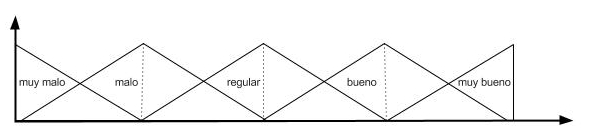
\includegraphics[width=15cm]{graficas/variables.jpg}
\end{grafico}
La adopción de variables lingüísticas recientemente se ha generalizado y se utiliza para evaluar las calificaciones lingüísticas dadas por los evaluadores. Por otra parte, las variables lingüísticas se emplean también como una forma de medir el logro del valor de rendimiento para cada criterio.\\
\\
El término de “conjunto difuso” (o conjunto borroso), aparece por primera vez en los años sesenta cuando el profesor Lotfi A. \citet{zadeh1965fuzzy}, de la Universidad de Berkeley en USA, publica un artículo titulado ``Fuzzy sets''. Luego de esta publicación, Zadeh ha iniciado líneas de investigación fundamentales sobre el análisis de sistemas complejos y los procesos de toma de decisiones, la lógica difusa y sus implicaciones en diversos dominios tales como el razonamiento aproximado, la gestión de la incertidumbre, los sistemas expertos, las redes neuronales, la información granular y su centralidad en el razonamiento humano, la computación con palabras.
Por ejemplo, se consulta un grupo de personas y se establecen las funciones de pertenencia para las temperaturas ``fría'', ``normal'' y ``caliente'' que se representan mediante conjuntos difusos; y se obtiene como resultado lo indicado en el \refgrafico{graficoTemperaturas}:

\begin{grafico}[titulo = Funciones de pertenencia para algunas temperaturas, etiqueta=graficoTemperaturas]
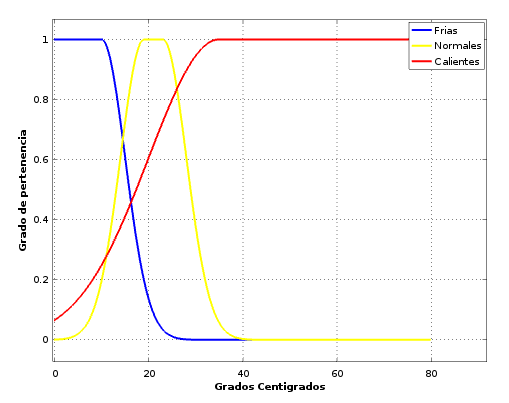
\includegraphics[width=12cm]{graficas/temparaturas.png}
\end{grafico}
Se observa que para el caso de temperatura ``normal'', en la región alrededor de 22º C se tiene un grado de pertenencia igual a 1, mientras que para valores menores o iguales a 10º C y mayores o iguales a 40º C, el grado de pertenencia es cero.\\
\\
Entre los tipos de funciones de pertenencia que más se usan en la especificación de números difusos están las de forma triangular, trapezoidal, gaussiana y de campana generalizada, las cuales pueden definirse de manera conveniente y concisa mediante fórmulas matemáticas parametrizadas \cite[]{jang1997neuro}. El \refcuadro{tablaModeloDM} muestra las fórmulas y parámetros de estas funciones.\\

\begin{cuadro}[titulo= Fórmulas y parámetros de funciones de pertenencia, etiqueta = tablaModeloDM]{|p{1.9cm}|c|c|}
\hline
\textbf{Tipo de Función} & \textbf{Fórmulas} & \textbf{Parámetros} \\
\hline
 & & \\
\textit{Triangular} & 
${ \mu  }_{ A }(x)=\left\{ \begin{matrix} 0\quad \quad \Leftrightarrow \quad (x\le a\quad \vee \quad x\ge c) \\ \cfrac { x-a }{ b-a } \quad \quad \Leftrightarrow \quad \quad \quad a\le x\le b \\ \cfrac { c-x }{ c-b } \quad \quad \Leftrightarrow \quad \quad \quad b\le x\le c\quad  \end{matrix} \right $
& $a, b, c$ \\
 & & \\
\textit{Trapezoidal} &
 ${ \mu  }_{ A }(x)=\left\{ \begin{matrix} 0\quad \quad \Leftrightarrow \quad (x\le a\quad \vee \quad x\ge d) \\ \cfrac { x-a }{ b-a } \quad \Leftrightarrow \quad \quad  a\le x\le b \\ 1\quad \quad \quad  \Leftrightarrow \quad \quad b\le x\le c \\ \cfrac { d-x }{ d-c } \quad \Leftrightarrow \quad  \quad c\le x\le d\quad  \end{matrix} \right $ 
 & $a, b, c, d$ \\
 & & \\
\textit{Gaussiana} 
& 
${ \mu  }_{ A }(x)={ e }^{ -{ 1 }/{ 2 }{ ((x-c)-\sigma ) }^{ 2 } }$
& $c, \sigma$\\ 
 & & \\
\textit{Campana generalizada}
& 
${ \mu  }_{ A }(x)=\cfrac { 1 }{ 1+{ \left| \cfrac { x-c }{ a }  \right|  }^{ 2b } }$
& $a, b, c$\\
 & & \\
 \hline
\end{cuadro}
\fuentecuadro{3}{ \citet[pp. 25-26]{jang2002neuro}}
\subseccion{Relaciones y operaciones básicas entre conjuntos difusos}

A continuación se describen dos relaciones y cuatro operaciones estandarizadas, con base en dos conjuntos difusos cualesquiera $A, B$ en el mismo universo $X$ \cite[pp. 21-23]{jang2002neuro}.

\subsubseccion{Igualdad}
 Se dice que $A$ es igual a $B$ si y sólo si para cada elemento $x \in X$, los números reales $\mu_{A}(x)$ y $\mu_{B}(x)$ son iguales. Se denota $A = B$.
\subsubseccion{Subconjunto}
Se dice que $A$ es un subconjunto de $B$ si y sólo si para cada elemento $x \in X$, el número real  $\mu_{A}(x)$  es menor que el número real  $\mu_{B}(x)$   , o ambos números reales son iguales. Se denota $A \subseteq B$.
\subsubseccion{Unión}
La unión estándar de $A$ y $B$ es el conjunto difuso $C$ en $X$, tal que su función de pertenencia $\mu_{C}:X \rightarrow [0, 1]$ está definida por $\mu_{C}(x)=\max {{\{\mu_{A}(x),\mu_{B}(x)\}}}$ para cada $x \in X$. Se denota $A \cup B$. \\
El \refgrafico{graficoUnion} muestra la unión estándar de dos conjuntos difusos con funciones de pertenencia triangulares.
\begin{grafico}[titulo = Union estandar en conjuntos difusos, etiqueta=graficoUnion]
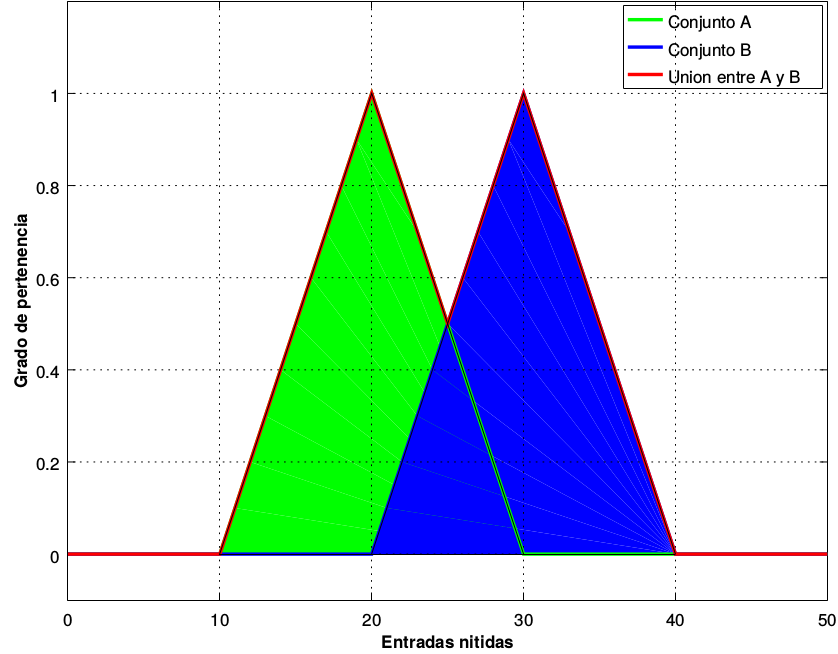
\includegraphics[width=8cm]{graficas/union.png}
\end{grafico}
\subsubseccion{Intersección}
La intersección estándar de $A$ y $B$ es el conjunto difuso $C$ en $X$, tal que su función de pertenencia $\mu_{C}(x):X \rightarrow [0, 1]$ está definida mediante la proposición $\mu_{C}= \min \{\mu_{A}(x), \mu_{B}(x) \}$ para cada $x \in X$. Se denota $A \cap B$.\\
El \refgrafico{graficoInterseccion} muestra la intersección estándar entre dos conjuntos difusos con funciones de pertenencia triangulares.
\begin{grafico}[titulo = Intersección estandar en conjuntos difusos, etiqueta = graficoInterseccion]
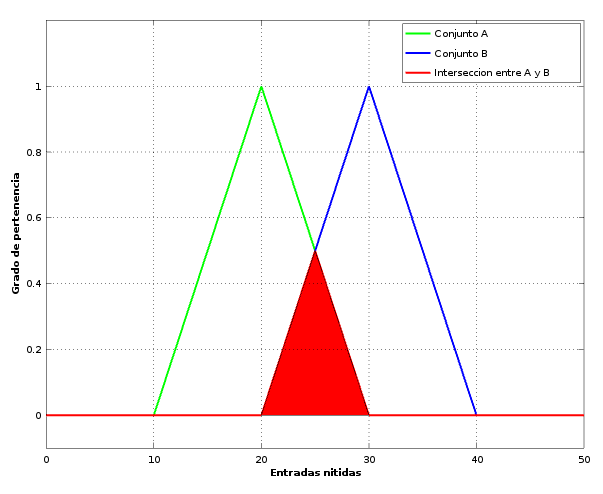
\includegraphics[width=8cm]{graficas/interseccion.png}
\end{grafico}
\subsubseccion{Complemento}
El complemento estándar de $A$ es el conjunto difuso $C$ en $X$, tal que su función de pertenencia $\mu_{C}(x):X \rightarrow [0, 1]$ está definida por $\mu_{C}(x)=1 -\mu_{A}(x)$ para cada $x \in X$. Se denota $\bar{A}$.\\
El \refgrafico{graficoComplemento} muestra el complemento estándar de un conjunto difuso con función de pertenencia triangular.
\begin{grafico}[titulo = Complemento estandar en conjuntos difusos, etiqueta = graficoComplemento]
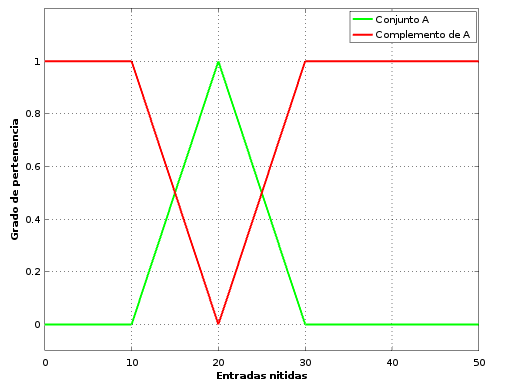
\includegraphics[width=8cm]{graficas/complemento.png}
\end{grafico}
\subsubseccion{Diferencia}
La diferencia estándar de $A$ y $B$ es el conjunto borroso $C$ en $X$, tal que su función de pertenencia $\mu_{C}(x):X \rightarrow [0, 1]$ está definida por medio de la proposición $\mu_{C}= \min \{\mu_{A}(x), 1 - \mu_{B}(x) \}$  para cada $x \in X$. Se denota $A-B$.
El \refgrafico{graficoDiferencia} muestra la diferencia estándar de dos conjuntos borrosos con funciones de pertenencia trapezoidales:
\begin{grafico}[titulo = Diferencia estandar en conjuntos difusos, etiqueta = graficoDiferencia]
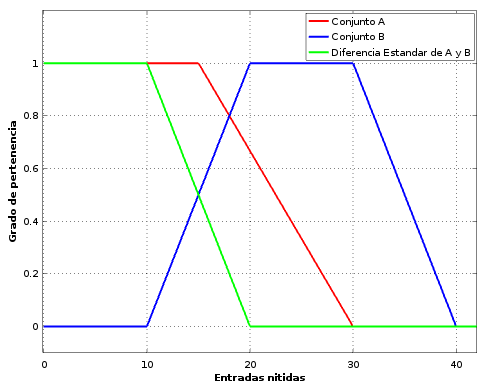
\includegraphics[width=8cm]{graficas/diferencia.png}
\end{grafico}
\\
Puesto que $\min \{\mu_{A}(x), 1 - \mu_{B}(x)\} = \min \{\mu_{A}(x), \mu_{\bar{B}}(x)\} =\mu_{A \cap \bar{B} }(x)$, entonces $(\forall x \in X)[\mu_{A - B }(x) = \mu_{A \cap \bar{B} }(x)]$.
\\
Luego, $A - B = A \cap \bar{B}$, es decir, la diferencia estándar de $A$ y $B$ es el conjunto difuso que se obtiene mediante la intersección estándar de $A$ y el complemento de $B$.
\subseccion{Lógica difusa y variables lingüísticas}
El término ``lógica difusa'' ha sido utilizado con dos significados diferentes. En un sentido conceptual, se refiere a un sistema lógico que generaliza la lógica clásica bivalente, para razonamiento bajo incertidumbre. En un sentido procedimental, la lógica difusa se refiere a los métodos y las técnicas que emplean conjuntos borrosos.\\
\\
La lógica difusa tiene una faceta relacional, que trata principalmente de la
representación y manipulación de funciones y relaciones definidas en forma
imprecisa. Esta faceta es fundamental en aplicaciones en áreas de información, control automático y modelado de sistemas. La lógica difusa es considerada como un campo de estudio dentro de la Inteligencia Artificial \cite[]{yen1999fuzzy}. La lógica difusa permite desarrollar sistemas y tecnologías computacionales con un manejo adecuado de incertidumbre en la información para realizar razonamientos y resolver problemas que requieran de inteligencia.\\
\\
\citet{trillas1992aplicaciones},  afirman que la lógica difusa permite representar el conocimiento común en un lenguaje matemático especial (el de la teoría de los subconjuntos borrosos y las distribuciones de posibilidad a ellos asociadas) y, a través de un cálculo lógico que flexibiliza la noción operativa de verdad, vista como predicado singular, permite efectuar inferencias aproximadas a partir de patrones de razonamiento que reproducen, aceptablemente, los métodos usuales de razonamiento que son, mayoritariamente, de tipo lingüístico cualitativo y no necesariamente cuantitativos. Por descontado, con posibilidad de reinterpretación de los resultados finales obtenidos a través de fórmulas, es un auxiliar común que presentan las matemáticas.\\
Una variable lingüística \cite[]{zadeh1975concept} es una $5-upla(x, T_{x}, U, G, M)$, en la cual:
\begin{viñetas}
\item $x$ es el nombre de la variable.
\item $T_{x}$ es el conjunto de términos lingüísticos referidos a la variable $x$.
\item $U$ es el universo del discurso en el contexto de la variable $x$.
\item $G$ es una regla sintáctica para generar los nombres de valores de $x$. 
\item $M: \rightarrow \F (U)$ es la regla semántica que asigna a cada término lingüístico $t \in T_{x}$ su significado. $M(t) \in \F (U)$, siendo $\F (U)$ la familia de conjuntos borrosos en $\mathbb{R}$.
\end{viñetas}

\subseccion{Medidas de comparación entre conjuntos borrosos}
\\
\citet{zadeh1971similarity}, define la noción de similitud (similarity) como la generalización de la noción de equivalencia. Los conjuntos borrosos son utilizados en las mediciones de similitudes y disimilitudes entre objetos por su capacidad de representar información subjetiva resultante de la complejidad del mundo real. Las medidas de similitud entre conjuntos borrosos pueden tener una motivación de teoría de conjuntos o una motivación geométrica. Entonces, las medidas de similitud se pueden distinguir en dos clases: la basada en teoría de conjuntos y la geométrica.
A continuación, se hace una descripción de medidas de similitud entre conjuntos borrosos para cada una de estas clases.

\subseccion{Comparación de Objetos con Atributos Difusos}
La comparación y descripción de objetos es una operación habitual en muchos dominios: psicología, analogía, ciencias físicas, procesamiento de imágenes, agrupamiento (``clustering''), razonamiento deductivo, razonamientos basados en casos, entre otros campos. Estas comparaciones frecuentemente se basan en medidas que intentan determinar qué puntos tienen en común ambos objetos, es decir, medidas de similitud \cite[]{bouchon2008similarities}.\\
\\
La comparación de objetos con descripciones imperfectas, afectadas con imprecisiones e inexactitudes, puede ser tratada utilizando conjuntos borrosos para representar tales descripciones.

\subseccion{Toma de decisiones con múltiples atributos}
El proceso de toma de decisiones implica una serie de pasos: identificación de los problemas, construcción de preferencias, evaluación de las alternativas, y determinación de las mejores alternativas \cite[]{simon1977causal, kleindorfer1993decision}.\\
En general, tres tipos de análisis formal pueden emplearse para resolver problemas de toma de decisiones \cite[]{bell1988descriptive, kleindorfer1993decision}:
\\
\begin{viñetas}
\item El análisis descriptivo, que se ocupa de los problemas donde los decisores (``Decision Makers'', DM) ofrecen soluciones particulares.
\item El análisis prescriptivo, el cual considera que los métodos DM deben utilizarse para mejorar sus decisiones.
\item El análisis normativo se centra en los problemas que los DM idealmente deberían abordar.
\\
\end{viñetas}
La toma de decisiones es muy intuitiva al considerar los problemas de un criterio único, ya que sólo hay que elegir la alternativa con la calificación de preferencia más alta. Sin embargo, cuando el DM evalúa alternativas con múltiples criterios, aparecen muchos problemas, tales como los pesos de los criterios de preferencia, la dependencia, y los conflictos entre los criterios, parecen complicar los problemas y necesitan ser superadas por métodos más sofisticados.\\
\\
Con el fin de hacer frente a los problemas MCDM, el primer paso es averiguar cuántos atributos o criterios existen en el problema y la forma de entender los problemas (es decir, la identificación de los problemas). A continuación, se debe recolectar los datos o informaciones adecuadas en las que las preferencias de DM se pueden reflejar correctamente (es decir, la construcción de las preferencias).  Posteriormente se requiere construir un conjunto de posibles alternativas o estrategias con el fin de garantizar que se alcance el objetivo (es decir, la evaluación de las alternativas). Finalmente se selecciona un método apropiado para ayudar a evaluar y posicionar las alternativas o estrategias (es decir, encontrar y determinar la mejor alternativa).\\
\\
A continuación se presentan algunos métodos para la evaluación de sistemas de información: 

\subsubseccion{Medidas globales de similitud}
Más de un atributo puede ser comparado entre dos casos. El algoritmo aplicado cuando hay más de un atributo relevante, debe ser considerado. En esta situación, se puede calcular la similitud promedio ponderada \cite[]{pal2004foundations}. Si SM denota una medida global de similitud, se tendrá la siguiente fórmula:
\begin{ecuacion}{ecuacionMedidaSimilitud}
	{S}_{M}=\cfrac {\sum _{i=1}^{ n }{ { w }_{ { M }_{ i } }}}{\sum _{ i=1 }^{ n }{ { w }_{ i }}}
\end{ecuacion}
Donde $S_{M_{i}}$ es la $i-ésima$ medida local de similitud, y $w_{i}$ es un factor de peso asociado con la $i-ésima$ medida local de similitud que es proporcional a la importancia relativa que se le asigne al atributo relacionado.

\subsubseccion{Proceso Analítico Jerárquico (AHP)}
Es una técnica estructurada para tratar con decisiones complejas. En lugar de prescribir la decisión “correcta”, el AHP ayuda a los decisores a encontrar la solución que mejor se ajusta a sus necesidades y a su comprensión del problema. \citet{bernoulli1783sammlung} propuso el concepto de función de utilidad para reflejar búsqueda humana, como la máxima satisfacción, \citet{neumann1947theory}  presentaron la teoría del juego y modelo de comportamiento económico, que amplió los estudios sobre los  problemas del  comportamiento económico humano para la Toma de Decisiones con Atributos Múltiples (“Multiple Attribute Decision Making”, MADM), una cantidad cada vez mayor de la literatura se ha dedicado a este campo. En términos generales, los procedimientos de MADM pueden resumirse en seis pasos a saber \cite[]{dubois1980systems}:
\begin{viñetas}
\item \textbf{Paso 1:} Definir la naturaleza del problema.
\item \textbf{Paso 2:} Construir un sistema jerárquico para su evaluación (gráfica). 
\item \textbf{Paso 3:} Seleccionar el modelo de evaluación apropiada.
\item \textbf{Paso 4:} Obtener los pesos relativos y puntuación de rendimiento de cada atributo con respecto a cada alternativa.
\item \textbf{Paso 5:} Determinar la mejor alternativa de acuerdo con los valores de utilidad, que son el valor agregado de los pesos relativos, y las puntuaciones de rendimiento correspondiente a las alternativas.
\\
\end{viñetas}
Cabe destacar que \citet{keeney1976decision} sugieren cinco principios que deben seguirse para la formulación de los criterios: 
(1) La integridad, (2) La operatividad, (3) de descomposición, (4) no redundancia, y (5) tamaño mínimo .
\subsubsection{Método de valores propios}
AHP fue propuesto por \citet{saaty1977scaling} para modelar los procesos de toma de decisiones subjetivas basadas en múltiples atributos en un sistema jerárquico. A partir de ese momento, se ha utilizado ampliamente en la planificación empresarial, la selección de portafolios, y el análisis de costo/beneficio por las agencias gubernamentales para fines de asignación de recursos. Cabe destacar que todos los problemas de decisión se consideran como una estructura jerárquica en el AHP. El primer nivel indica el objetivo para el problema de decisión específico. En el segundo nivel, el objetivo se descompone de varios criterios y los niveles más bajos puede seguir este principio a dividirse en otros subcriterios. Por lo tanto, la forma general de la AHP se puede representar como se muestra en el \refgrafico{graficoAHP}.
\begin{grafico}[titulo = Forma general de la AHP, etiqueta=graficoAHP]
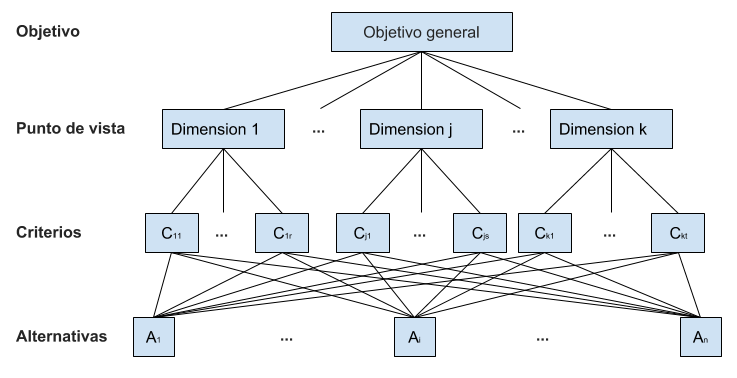
\includegraphics[width=15cm]{graficas/AHP.png}
\end{grafico}
\subsubseccion{Escala de proporción en el AHP}El \refcuadro{tablaEscalaAHP} representa la escala de índices que se emplea para comparar el peso entre los criterios de importancia de acuerdo con el significado lingüístico de 1 a 9 para denotar desde la misma importancia(1) a la extrema importancia(9).
\begin{cuadro}[titulo= Escala de proporción en el AHP, etiqueta=tablaEscalaAHP]{|p{1.8cm}|c|c|c|c|c|p{2cm}|}
\hline
Intensidad  & 1 & 3 & 5 & 7 & 9 & 2,4,6,8 \\
\hline
Termino lingüístico & Igual & Moderada & Fuerte & Demostrada & Extrema & Valores intermedios \\
\hline
\end{cuadro}
Además, con el fin de garantizar la coherencia de la percepción subjetiva y la exactitud de los pesos comparativos, se sugieren dos índices, el índice de consistencia (“Consistency Index”, $CI$) y el radio de consistencia (“Consistency Ratio” , $CR$). La ecuación del $CI$ se puede expresar como:
\begin{ecuacion}{ecuacionCI}
C.I.=\cfrac { (\mu _{ \max}-n)}{(n-1)}
\end{ecuacion}
Donde $\mu_{ \max}$ es el valor propio más grande, y $n$	 representa los números de los atributos. \citet{saaty1980analytic} sugirió que el valor del $CI$ no debe exceder de $0,1$ para un resultado confiable. Por otro lado, la $CR$ se puede calcular como:
\begin{ecuacion}{ecuacionCR}
C.R.=\cfrac {C.I.}{R.I.}
\end{ecuacion}
El índice aleatorio (“Random Index”, $R.I.$) para diferentes tamaños matriciales se puede apreciar en el \refcuadro{tablaEscalaProporcionAHP}.
\begin{cuadro}[titulo= Valor de RI para diferentes numeros de entradas(n) , etiqueta = tablaEscalaProporcionAHP]{|l|l|l|l|l|l|l|l|l|l|l|l|}
\hline
$n$ & 3 & 4 & 5 & 6 & 7 & 8 & 9 & 10 & 11 & 12 & 13 \\
\hline
R.I. &  0.52 & 0.89 & 1.11 & 1.25 & 1.35 & 1.40 & 1.45 & 1.49 & 1.51 & 1.54 & 1.56
  \\
\hline
\end{cuadro}
El $C.R.$ debe ser inferior a 0,1 para obtener un resultado fiable y 0,2 es el nivel máximo tolerado.\\
\\
En las aplicaciones a menudo es conveniente trabajar con números difusos triangulares debido a su simplicidad computacional y son útiles en la promoción de la representación y tratamiento de la información en un entorno difusa. 
\subsubseccion{Integración de AHP con los conjuntos difusos}
La metodología AHP Difusa considera la incorporación de números difusos, donde por conveniencia se utilizan números difusos triangulares (``Triangular Fuzzy Numbers'' ,TFN) debido a su simplicidad computacional. Inicialmente utiliza los números difusos para indicar el nivel 	de intensidad o importancia relativa que un factor de la jerarquía tiene por sobre otro. A partir de estas comparaciones se construye la matriz de comparaciones con números triangulares.
\begin{ecuacion}{ecuacionMatriz}
\tilde { A } = \begin{bmatrix} 1 & \tilde { { a } }_{ 12 }  & ... & \tilde { { a } }_{ 1n }  \\ \tilde { { a } }_{ 21 }  & 1 & ... & \tilde { { a }}_{ 2n }   \\ ... & ... & ... & ... \\ \tilde { { a } }_{ n1 }  & ... & ... & 1 \end{bmatrix}
\end{ecuacion}
Donde, $\tilde {{a}}_{ij}$ es un número triangular difuso, $\tilde {{a}}_{ij} = (l_{ij}, m_{ij}, n_(ij))$,   $\tilde {{a}}_{ji}=1/\tilde {{a}}_{ij}$. Para cada $TFN$, $\tilde {{a}}_{ij}$ o $M=(l, m, n)$, Es función de pertenencia de  $\tilde {{a}}_{ij}(x)$  o $M(x)$, siendo $-\infty \leq x \leq \infty$ para el intervalo cerrado $[0, 1]$.\\
\\
La mejor alternativa es obtenida consecuentemente a partir de un sistema de clasificación para números difusos.  El método AHP es un método que permite atribuir pesos donde valores numéricos no pueden ser obtenidos directamente. Este método trabaja a partir de una matriz donde se localizan las comparaciones entre pares, según la importancia o preponderancia relativa que un elemento de la jerarquía tenga sobre otro.


\subsubseccion{Técnica para el orden de preferencia por similitud con solución ideal (TOPSIS)}

El método TOPSIS es un modelo de decisión propuesto para ordenar preferencias por similitud con una solución ideal, es por tanto un método de clasificación (ranking). Fue desarrollado por \citet{hwang1981lecture} y mejorada por los autores \citet{chen1992fuzzy}, también trabajaron \citet{zeleny1994search}, \citet{lai1994topsis}, \citet{garcia2012rank} entre otros. TOPSIS es un método de decisión multicriterio de ordenación para identificar las soluciones de un conjunto finito de alternativas. El principio básico es que la alternativa elegida debe tener la menor distancia a la solución ideal positiva y la mayor distancia a la solución ideal negativa. Una solución ideal se define como una colección de puntuaciones o valores en todos los atributos considerados en la decisión, pudiendo suceder que tal solución sea inalcanzable. El vector compuesto por los mejores valores del j-ésimo atributo respecto de todas las alternativas posibles es quien recibe el nombre de ``solución ideal positiva'' (SIP); recíprocamente, la ``solución ideal negativa'' (SIN) será aquella cuyo vector contenga los peores valores en todos los atributos. A fin de definir la solución ideal, el método  TOPSIS establece un índice de similaridad que se construye combinando la proximidad al ideal positivo y la lejanía respecto al ideal negativo. El procedimiento de TOPSIS puede expresarse en una serie de pasos que pueden verse en \citet{jahanshahloo2006algorithmic}, y se describen a continuación.\\
Calcular la matriz de decisión normalizado. El valor de $n_{ji}$ normalizado se calcula como
\begin{ecuacion}{ecuacionNormalizacion}
n_{ ij }=\cfrac { x_{ ij } }{ \sqrt { \sum _{ i=1 }^{ n }{ { x }_{ ij }^{ 2 }\quad ,\quad i = 1,\quad 2,\quad ...,\quad m;\quad j = 1,\quad 2,\quad ...,n }  }  } 
\end{ecuacion}
Luego, calcular la matriz de decisión de pesos normalizados. Los pesos normalizados $v_{ij}$ son calculados como
$v_{ij}=w_{ij}n_{ij}; i=1, 2,..., m; j=1,2,..., n$
donde  $w_{j}$ es el peso del $i-ésimo$ atributo o criterio, y
\begin{ecuacion}{ecuacionPesoICriterio}
\sum _{ j=1 }^{ n }{ w_{ i } } =1
\end{ecuacion}

Determinar la solución ideal positiva y la solución ideal negativa:
\begin{ecuaciones}
{ A }^{ + }=\{ { v }_{ 1 }^{ + },\quad { v }_{ 2 }^{ + },\quad ...,\quad { v }_{ n }^{ + }\} =\left\{ ({ max }_{ j }v_{ ij }|i\in I),\quad ({ min }_{ j }v_{ ij }|i\in J) \right\} \\
{ A }^{ - }=\{ { v }_{ 1 }^{ - },\quad { v }_{ 2 }^{ - },\quad ...,\quad { v }_{ n }^{ - }\} =\left\{ ({ min }_{ j }v_{ ij }|i\in I),\quad ({ max }_{ j }v_{ ij }|i\in J) \right\}
\end{ecuaciones}
Calcular las medidas de separación, usando la distancia Euclidiana $n-dimensional$. La separación de cada alternativa de la solución ideal, es dada como:\\
\begin{ecuacion}{ecuacionpositiva}
{ d }_{ i }^{ + }={ \left\{ \sum _{ j=1 }^{ n }{ { ({ v }_{ ij }-{ v }_{ i }^{ + }) }^{ 2 } }  \right\}  }^{ \sfrac { 1 }{ 2 }  };\quad i=1,2,\quad ...,m
\end{ecuacion}
Del mismo modo, la separación de la solución ideal negativa se da como:
\begin{ecuacion}{ecuacionpositiva}
{ d }_{ i }^{ - }={ \left\{ \sum _{ j=1 }^{ n }{ { ({ v }_{ ij }-{ v }_{ i }^{ - }) }^{ 2 } }  \right\}  }^{ \sfrac { 1 }{ 2 }  };\quad i=1,2,\quad ...,m
\end{ecuacion}
Calcular la cercanía relativa a la solución ideal. La proximidad relativa de la alternativa  $A_{i}$ con respecto a $A^{+}$ se define como
\begin{ecuacion}{ecuacioncercaniarelat}
{ R }_{ i }={ { d }_{ i }^{ - } }/{ ({ d }_{ i }^{ + }-{ d }_{ i }^{ - }),\quad i=1,2,\quad ...,\quad m }
\end{ecuacion}
Desde $d_{i} \geq 0$  y  $d_{i} \geq 0$ , entonces claramente, $R_{i}\in [0,1]$.\\
\\
Clasificar las alternativas utilizando este índice, permite el ordenamiento de las mismas respecto a las preferencias en forma descendente.  El principio básico del método TOPSIS es que la alternativa elegida debe tener la ``distancia más corta'' de la solución ideal positiva y el ``distancia más lejana'' de la solución ideal negativa.
\subseccion{Aplicaciones móviles y sus características}
\citet{santiago2015mobile} definen a las aplicaciones móviles como aplicaciones informáticas diseñadas para ser ejecutada en teléfonos inteligentes, tabletas y otros dispositivos móviles y que permite a los usuarios efectuar una tarea concreta de cualquier tipo ---profesional, de ocio, educativas, de acceso a servicios, entre otras---, facilitando las gestiones o actividades a desarrollar.
A nivel de programación, existen varias formas de desarrollar aplicaciones. Cada una de ellas tiene diferentes características y limitaciones, especialmente desde el punto de vista técnico.
\citet{cuello2013disenando} definen tres tipos de aplicaciones; las nativas, las web y las híbridas. A continuación se describe cada una de estas:  

\subsubseccion{Aplicaciones nativas}

Las aplicaciones nativas son aquellas que han sido desarrolladas con el software que ofrece cada sistema operativo a los programadores, llamado genéricamente Software Development Kit o SDK. Así, Android, iOS y Windows Phone tienen uno diferente y las aplicaciones nativas se diseñan y programan específicamente para cada plataforma, en el lenguaje utilizado por el SDK.\\
Este tipo de apps se descarga e instala desde las tiendas de aplicaciones ---con ciertas excepciones en el caso de Android, que veremos en el capítulo «Lanzando la app»--- sacando buen partido de las diferentes herramientas de promoción y marketing de cada una de ellas.\\
Las aplicaciones nativas se actualizan frecuentemente y en esos casos, el usuario debe volver a descargarlas para obtener la última versión, que a veces corrige errores o añade mejoras.
Una característica generalmente menospreciada de las apps nativas, es que pueden hacer uso de las notificaciones del sistema operativo para mostrar avisos importantes al usuario, aun cuando no se esté usando la aplicación, como, por ejemplo, los mensajes de Whatsapp.\\
Además, no requieren de Internet para funcionar, por lo que ofrecen una experiencia de uso más fluida y están realmente integradas al teléfono, lo cual les permite utilizar todas las características de hardware del terminal, como la cámara y los sensores (GPS, acelerómetro, giróscopo, entre otros).\\
A nivel de diseño, esta clase de aplicaciones tiene una interfaz basada en las guías de cada sistema operativo, logrando mayor coherencia y consistencia con el resto de aplicaciones y con el propio SO. Esto favorece la usabilidad y beneficia directamente al usuario que encuentra interfaces familiares.\\

\subsubseccion{Aplicaciones web}

La base de programación de las aplicaciones web -también llamadas webapps- es el HTML, conjuntamente con JavaScript y CSS, herramientas ya conocidas para los programadores web.
En este caso no se emplea un SDK, lo cual permite programar de forma independiente al sistema operativo en el cual se usará la aplicación. Por eso, estas aplicaciones pueden ser fácilmente utilizadas en diferentes plataformas sin mayores inconvenientes y sin necesidad de desarrollar un código diferente para cada caso particular.
Las aplicaciones web no necesitan instalarse, ya que se visualizan usando el navegador del teléfono como un sitio web normal. Por esta misma razón, no se distribuyen en una tienda de aplicaciones, sino que se comercializan y promocionan de forma independiente.\\
Al tratarse de aplicaciones que funcionan sobre la web, no es necesario que el usuario reciba actualizaciones, ya que siempre va a estar viendo la última versión. Pero, a diferencia de las apps nativas, requieren de una conexión a Internet para funcionar correctamente.\\
Adicionalmente, tienen algunas restricciones e inconvenientes en factores importantes como gestión de memoria y no permiten aprovechar al máximo la potencia de los diferentes componentes de hardware del teléfono.
Las aplicaciones web suelen tener una interfaz más genérica e independiente de la apariencia del sistema operativo, por lo que la experiencia de identificación del usuario con los elementos de navegación e interacción, suele ser menor que en el caso de las nativas.

\subsubseccion{Aplicaciones hibridas}
Este tipo de aplicaciones es una especie de combinación entre las dos anteriores. La forma de desarrollarlas es parecida a la de una aplicación web ---usando HTML, CSS y JavaScript---, y una vez que la aplicación está terminada, se compila o empaqueta de forma tal, que el resultado final es como si se tratara de una aplicación nativa.
Esto permite casi con un mismo código obtener diferentes aplicaciones, por ejemplo, para Android y iOS, y distribuirlas en cada una de sus tiendas.
A diferencia de las aplicaciones web, éstas permiten acceder, usando librerías, a las capacidades del teléfono, tal como lo haría una app nativa.2
Las aplicaciones híbridas, también tienen un diseño visual que no se identifica en gran medida con el del sistema operativo. Sin embargo, hay formas de usar controles y botones nativos de cada plataforma para apegarse más a la estética propia de cada una.
Existen algunas herramientas para desarrollar este tipo de aplicaciones. Apache Cordova3 es una de las más populares, pero hay otras, como Icenium4, que tienen la misma finalidad.
\subsubseccion{Desarrollo de aplicaciones móviles}
De acuerdo con \citet{wasserman2010software} en muchos aspectos, el desarrollo de aplicaciones móviles es similar a la ingeniería de software para otros tipos de aplicaciones. Problemas comunes incluyen la integración con el hardware del dispositivo, así como los problemas tradicionales de la seguridad, el rendimiento, la fiabilidad y las limitaciones de almacenamiento. Sin embargo, las aplicaciones móviles presentan algunos requisitos adicionales que se encuentran menos comúnmente en aplicaciones de software tradicionales, incluyendo:
\begin{enumeracion}
\item Posible interacción con otras aplicaciones - los dispositivos más integrados sólo tienen software instalado de fábrica, pero los dispositivos móviles pueden tener numerosas aplicaciones de diversas fuentes, con la posibilidad de interacciones entre ellos.
\item La manipulación del sensor - los dispositivos móviles más modernos, por ejemplo, ``teléfonos inteligentes'', incluyen un acelerómetro que responde al movimiento del dispositivo, una pantalla táctil que responde a numerosos gestos, junto con los bienes y / o teclados virtuales, un sistema de posicionamiento global, un micrófono utilizable por aplicaciones distintas de las llamadas de voz, una o más cámaras, y protocolos de red múltiples.
\item Aplicaciones nativas e híbridas (web móvil) - dispositivos más integrados utilizan sólo las instaladas directamente en el dispositivo de software, pero los dispositivos móviles a menudo incluyen aplicaciones que invocan servicios a través de la red telefónica o Internet a través de un navegador web y afectan a los datos en el dispositivo.
\item Familias de plataformas de hardware y software - la mayoría de dispositivos embebidos ejecutan código que está hecho a la medida para las propiedades de ese dispositivo, pero los dispositivos móviles pueden tener que soportar las aplicaciones que se han escrito para todos los variados dispositivos que soportan el sistema operativo, y también para diferentes versiones del sistema operativo. Un desarrollador de Android, por ejemplo, debe decidir si se ha de construir una aplicación única o múltiples versiones para correr en la amplia gama de dispositivos Android y versiones del sistema operativo.
\item Seguridad - los dispositivos más integrados son ``cerrados'', en el sentido de que no hay manera fácil de atacar el software embebido y afectar a su funcionamiento, pero las plataformas móviles están abiertas, permitiendo la instalación de nuevas aplicaciones, y un ``malware'' puede afectar el funcionamiento global del dispositivo, incluida la transmisión encubierta de datos locales por una aplicación de este tipo.
\item Las interfaces de usuario - con una aplicación embebida hecha a la medida, el desarrollador puede controlar todos los aspectos de la experiencia del usuario, pero en una aplicación móvil deben compartir elementos comunes de la interfaz de usuario con otras aplicaciones y deben adherirse a lo desarrollado externamente para las directrices de la interfaz de usuario, muchas de las cuales se implementan en los kits de desarrollo de software (``Software development kit'', SDK) que forman parte de la plataforma.
\item Complejidad de las pruebas - mientras que las aplicaciones nativas se pueden probar de forma tradicional o a través de un emulador basado en PC, las aplicaciones web móviles son particularmente difíciles de probar. No sólo tienen muchos de los mismos problemas que se encuentran en aplicaciones de pruebas web; que además tienen problemas asociados con la transmisión a través de pasarelas y la red telefónica.
\item Consumo de energía - muchos aspectos de una aplicación afecta el consumo de energía del dispositivo y por lo tanto la duración de la batería. Dispositivos dedicados pueden ser optimizados para una máxima duración de la batería, pero las aplicaciones móviles pueden inadvertidamente hacer un uso extensivo de los recursos del consumo de batería.


\end{enumeracion}

%Si se va a usar el glosario
%\hacerglosario

	%!TEX root = ../trabajo.tex
\capitulo{Marco Metodológico}
A continuación se explicarán los aspectos metodológicos que se emplearán para la consecución de los objetivos específicos planteados. 

\seccion{Tipo de Investigación}
\citet{simon1996sciences}, consideró el diseño como un proceso científico, dada la necesidad existente de un método general que sea utilizado para diseñar o proyectar; a esta ciencia del diseño, la denominó ciencia de lo artificial, que es distinta del campo de las Ciencias de la Naturaleza y diferente también del ámbito de las Ciencias Sociales \cite[pp. 42-43]{gonzalez2007configuracion}. \citet[pp. 567-569]{hurtado2012metodologia}, afirma que en algunos contextos, a la investigación proyectiva también se le llama investigación tecnológica, estas  investigaciones conducen a inventos, programas, diseños o creaciones dirigidas a cubrir una determinada necesidad.
\\
\\ 
Desde otro ángulo, \citet{cordoba2005investigacion} afirma que las perspectivas metodológicas de la investigación en lo social ocurren de dos (2) maneras, estas son la cuantitativa y la cualitativa, pero si se parte de que existe la necesidad de transformar, entonces ni lo cuantitativo ni lo cualitativo son suficientes, de allí que se recurra a lo tecnológico. Definiendo a la investigación tecnológica como aquella que tiene por fin obtener un conocimiento para lograr modificar la realidad en estudio, vinculando la investigación y la transformación. La investigación tecnológica, denominada también como investigar, idear e innovar, persigue un conocimiento práctico, que sea más un conjunto de instrucciones a seguir para transformar el objeto, que explicaciones teóricas respecto a las cualidades del mismo. \\
\\
Esta investigación se desarrollará desde la perspectiva de la investigación tecnológica con un enfoque en ciencia del diseño, bajo la modalidad de investigación de Estudios de Proyectos, según el Manual para la Elaboración del Trabajo Conducente a Grado Académico de Especialización, Maestría y Doctorado,\citet[p. 63]{UCLAmanual2002}, donde se define de la siguiente manera:
\begin{citatextual}
`` Se entenderá por estudios de proyectos una proposición sustentada en un modelo viable para resolver un problema práctico planteado, tendente a satisfacer necesidades institucionales o sociales y pueden referirse a la formulación de políticas, programas, tecnología, métodos y procesos''.
\end{citatextual}
\\
Adicionalmente se destaca que el presente estudio se fundamentará en investigación monográfica documental.

\seccion{Diseño de la Investigación}

El término diseño de investigación se refiere al plan o estrategia que se desarrolla para obtener la información que se requiere en una investigación y responder al planteamiento \cite[p. 128]{hernandez2010metodologia}. Debido a las diferencias que radican en la naturaleza de las Ingenierías, incluída  las presentes en el  trabajo de toma de decisiones en proyectos de aplicaciones móviles con atributos difusos, respecto de otras disciplinas empíricas y formales, dificultan la aplicación directa de los métodos de investigación tradicionales. Teniendo en cuenta esta problemática, en el \refgrafico{graficoMetodologia} se muestra en forma esquemática el modelo del proceso de investigación en ciencia del diseño (``Design science research process'', DSRP) para producir y presentar investigación en sistemas de información \cite[p. 93]{peffers2006design}.\\
	
\begin{grafico}[titulo = Un modelo para producir y presentar investigación en ciencias del diseño, etiqueta=graficoMetodologia]
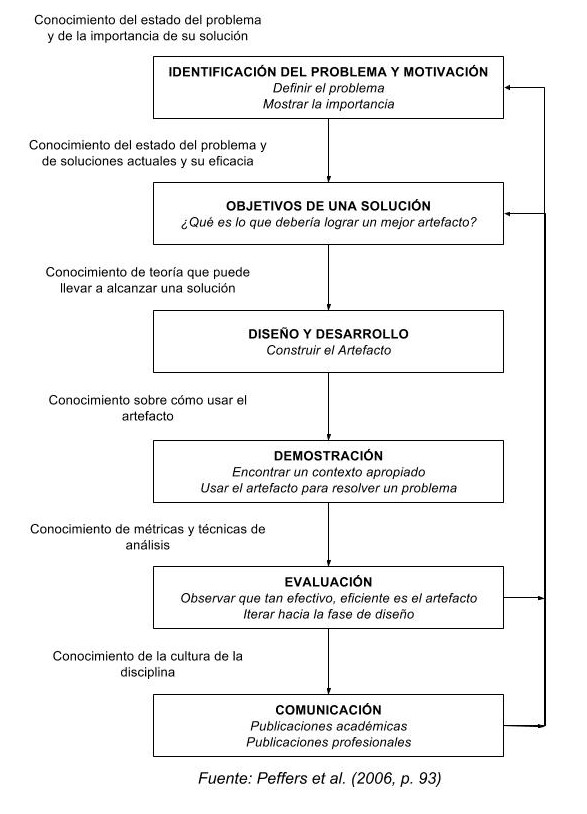
\includegraphics[width=11cm]{graficas/modeloMetodo.jpg}
\end{grafico}
Donde se destaca a \citet[pp. 1127-1128]{dresch2014design}, que apoyados en trabajos previos, entre ellos \citet{vaishnavi2015design} y \citet[p. 56]{peffers2006design}, han señalado que las etapas o pasos principales para realizar investigación basada el paradigma de Ciencia del Diseño, son: la conciencia del problema, sugerencia, desarrollo, evaluación, conclusión, y comunicación. Las salidas (resultados) y la descripción sucinta de dichos pasos se indican en el \refcuadro{tablaModeloCienciaD}, este procedimiento de investigación será utilizado en esta investigación.
\begin{cuadro}[titulo= Etapas principales para realizar investigación en ciencia de diseño, etiqueta = tablaModeloCienciaD]{|p{2cm}|p{4cm}|p{7cm}|}
\hline
 \textbf{Pasos del Proceso} & \textbf{Salidas} & \textbf{Descripción}\\
\hline
Conciencia del problema &
Propuesta 
(incluye formalización del problema, sus límites, y las soluciones que se consideran satisfactorias para el
problema)  &
Se identifica el problema de interés; el investigador debe tratar de comprender el problema para localizar todos sus aspectos y posibles interrelaciones con el contexto en el que está inserto.  \\
\hline
Sugerencia &
Diseño tentativo  &
Se produce un conjunto de posibles artefactos, y se selecciona uno de ellos.  \\
\hline
Desarrollo &
\textbf{Artefacto}  &
Se produce el artefacto, en su estado funcional.  \\
\hline
Evaluación & 
Medidas de desempeño & 
Busca determinar la forma precisa cómo se comporta el artefacto, verificando su habilidad para alcanzar el objetivo deseado. \\
\hline

Conclusiones &
 Resultados &
 Se sintetizan las etapas previas, detallando su proceso de conducción y justificando las elecciones realizadas por el investigador. \\
\hline
Comunicación &
Publicaciones y presentaciones académicas o profesionales (Informes, artículos, memorias, etc.) &
Presentar los resultados de la investigación a las audiencias apropiadas (comunidad académica y organizacional).  \\
\hline
\end{cuadro}
\\
\fuentecuadro{3}{\cite[]{dresch2014design}}\\
Para comprender el tipo de artefactos, \cite[]{lacerda2013design} indican que son objetos artificiales (es decir, creados por humanos), que pueden ser caracterizados en términos de objetivos, funciones y adaptaciones. Además, expresan que los artefactos pueden ser tipificados como: Constructos, Modelos, Métodos e Instanciaciones. Estos autores presentan descripciones de estos tipos de artefactos, como se reseña en el  \refcuadro{tablaArtefacto}.
\begin{cuadro}[titulo= Tipos de artefactos en ciencia de diseño, etiqueta = tablaArtefacto]{|p{4cm}|p{10cm}|}
\hline
 \textbf{Tipos de artefacto} & \textbf{Descripción} \\
\hline
Constructos & 
Constructos o conceptos forman parte del vocabulario de un dominio. Ellos constituyen una conceptualización utilizada para describir los problemas dentro del dominio y especificar las soluciones respectivas. \\
\hline
Modelos & 
Un modelo es un conjunto de proposiciones o declaraciones que expresan las relaciones entre los constructos. En actividades de diseño, los modelos representan situaciones como problema y solución. Puede ser visto como una descripción, o sea, como una representación de las cosas como son. Las ciencias naturales muchas veces usan el término ``modelo'' como sinónimo de ``teoría'', o ``modelos'' como teorías todavía incipientes. \\
\hline
\textbf{Métodos} & 
\textbf{Un método es un conjunto de pasos (un algoritmo u orientación) usado para ejecutar una tarea}. Los métodos se basan en un conjunto de constructos subyacentes (lenguaje) y una representación (modelo) en un espacio de solución. Los métodos pueden estar ligados a los modelos en el sentido de que los pasos pueden utilizar partes del modelo como una entrada que lo compone. \\
\hline
 Instanciaciones &
 Una instanciación es la concretización de un artefacto en su ambiente. Las instanciaciones operacionalizan constructos, modelos y métodos. Sin embargo, una instanciación puede realmente preceder la articulación completa de sus constructos, modelos y métodos subyacentes. Las instanciaciones demuestran la viabilidad y la eficacia de los modelos y métodos que ellas contienen.  \\
\hline
\end{cuadro}
\\
\fuentecuadro{3}{\cite[]{lacerda2013design}}\\

Por lo anteriormente mencionado, el tipo de artefacto a emplear es un método puesto del que se desarrollará un algoritmo conformado por un modelo para sistemas de información de criterios múltiples, utilizado en el área de aplicaciones móviles.

\seccion{Instrumentos de recolección de datos}
Para la recolección de datos, se empleará la técnica de revisión documental, la misma está orientada al tipo de investigación proyectiva. La revisión documental es un proceso que abarca la ubicación, recopilación, selección, revisión, análisis, extracción y registro de información contenida en documentos. Las técnicas de revisión documental pueden ser utilizadas como una vía para la recolección de datos durante una investigación de diseño documental o de fuente mixta, ya sea porque las unidades de estudio son documentos, o porque la información requerida para dar respuesta a la pregunta de investigación ya fue recolectada por otras personas y se encuentra consignada en archivos, registros o cualquier otro tipo de documento \cite[p. 851]{hurtado2012metodologia}. Dentro de las técnicas de revisión documental se utilizarán instrumentos tales como matrices de registro, fichas de observación y matrices de análisis \cite[pp. 855-859]{hurtado2012metodologia}.

\seccion{Instrumentos para el análisis y procesamiento de datos/información}

Para la presente investigación se aplicarán las bitácoras de análisis, técnica descrita por \citet[p.633]{hernandez2010metodologia}  como un instrumento invaluable para la validez y confiabilidad del análisis en información cualitativa. Para la comprobación del algoritmo se utilizará la técnica de simulación por computadora, con un software apropiado para producir las matrices de registros requeridas en esta investigación.\\
\\
Según \citet{hurtado2012metodologia}, la simulación es el proceso de diseñar y desarrollar un modelo computarizado de un sistema o proceso, para realizar experiencias que ayuden a entender el comportamiento del sistema, o evaluar varias estrategias con las cuales se puede operar el mismo. En consecuencia, para llevar a cabo la simulación por computadora, el investigador debe haber construido previamente un modelo explicativo del proceso o la situación a simular, y haberlo expresado en términos matemáticos. Para la creación de modelos, se utilizarán gráficas y fórmulas matemáticas, las técnicas de procesamiento y análisis de información. En el análisis se definirán las técnicas lógicas (inducción, deducción, análisis, síntesis), o estadísticas (descriptivas o inferenciales).

\seccion{Procedimiento de la Investigación}

En el siguiente procedimiento se describen las etapas o fases que se cumplirán para el desarrollo de cada objetivo específico, identificando en cada una de ellas las actividades involucradas y las técnicas a aplicar \cite[p. 11]{UNEXPOmanual2004}.
\begin{enumeracion}
\item[1. ]Para determinar los criterios que deben ser utilizados para la selección de proyectos de aplicaciones  móviles, se efectuarán las siguientes actividades:
\begin{enumeracion}
	\item[a) ] Realizar revisión documental sobre características de sistemas y tecnologías relacionados con la selección de proyectos para aplicaciones móviles.
	\item[b) ] Determinar los criterios representativos para la clasificación de proyectos mediate el uso de matriz de análisis. 
	\item[c) ] Describir los criterios que debe incluir el algoritmo a desarrollar.
\end{enumeracion}
\item[2. ] Para establecer las tareas que han de realizarse para la selección de proyectos de aplicaciones móviles utilizando criterios imprecisos, se hará lo siguiente:
\begin{enumeracion}
	\item[a) ]  Realizar revisión documental sobre métodos, sistemas y tecnologías 	referidos a la selección de proyectos de software en el desarrollo de nuevas aplicaciones móviles para identificar las tareas a incluir en la metodología a utilizar en el algoritmo propuesto.
	\item[b) ]  Describir las tareas que debe incluir el algoritmo a desarrollar.

\end{enumeracion}
\item[3. ]Para conformar el algoritmo que permita realizar las tareas definidas anteriormente, se efectuarán las siguientes actividades:
\begin{enumeracion}
	\item[a) ] Analizar sistemáticamente las tareas para definir los métodos apropiados para conformar el algoritmo propuesto. 
	\item[b) ] Conectar los métodos de manera que conformen un sistema coherente y ordenado. 
	\item[c) ] Especificar el método apropiado para llevar a cabo las tareas requeridas.
	\item[d) ] Validar el método especificado.
\end{enumeracion}

\item[4. ] Para evaluar el algoritmo propuesto, se realizarán las actividades señaladas a continuación:	
\begin{enumeracion}
	\item[a) ] Implementar 	un prototipo de sistema basado en el algoritmo propuesto. 
	\item[b) ]Elegir 	un caso representativo de selección de alternativas.
	\item[c) ]Realizar experimentos con el caso representativo, utilizando el prototipo de sistema basado en el algoritmo propuesta.
	\item[d) ]Analizar los resultados obtenidos del experimento realizado.
\end{enumeracion}
\item[5. ] Adicionalmente a las actividades anteriores, las cuales se efectúan para alcanzar los objetivos específicos, se llevará a cabo lo siguiente:
\begin{enumeracion}
	\item[a) ] Elaborar el Trabajo de Grado. 
	\item[b) ] Defender el Trabajo de Grado.
	\item[c) ] Elaborar la versión Final del Trabajo de Grado para optar al grado de Magíster Scientiarum
\end{enumeracion}
\end{enumeracion}
\\
A continuacion se ilustra el procedimiento de la presente investigación en el marco de la investigación de la ciencia del diseño, indicando las actividades por fases, así como las técnicas y procedimientos a utilizar, y los resultados parciales esperados.
\newpage
\subseccion{ Fase I. Determinar los criterios a incluir en el algoritmo}
\begin{cuadro}[sinleyenda, sinindice]{|p{6cm}|p{2.5cm}|p{4cm}|}
\hline
\textbf{Actividad  y/o Técnica} & \textbf{Instrumento} & \textbf{Resultado parcial esperado}\\
\hline
a) Realizar revisión documental sobre características de sistemas y tecnologías relacionados con la selección de proyectos para aplicaciones móviles.
 &  Revisión documental & Conocimiento sobre los criterios a incluir en el algoritmo a proponer.
  \\
  \hline
b)  Determinar los criterios representativos para la clasificación de proyectos. 
  & Lista de cotejo / Fichas de observación / Matrices de análisis 
  & Identificación de criterios a ser utilizados en el algoritmo. \\
  \hline
c) Describir los criterios que debe incluir el algoritmo a desarrollar. 
 &  Matrices de análisis
 & Información sobre características de los criterios a incluir \\
\hline
\end{cuadro}
\subseccion{ Fase II. Establecer las tareas a incluir en el algoritmo}

\begin{cuadro}[sinleyenda, sinindice]{|p{6cm}|p{2.5cm}|p{4cm}|}
\hline
\textbf{Actividad  y/o Técnica} & \textbf{Instrumento} & \textbf{Resultado parcial esperado}\\
\hline
d) Realizar revisión documental sobre métodos y sistemas relacionados con metodología a diseñar.
 & Revisión documental/ matrices de análisis de contenido
 & Conocimiento sobre las tareas a incluir en metodología a diseñar  \\
\hline
e) Describir las tareas a incluir 
 & Revisión documental/ matrices de análisis
 & Información sobre características de las tareas a incluir  \\
\hline
\end{cuadro}
\newpage
\subseccion{ Fase III. Conformación del algoritmo que permita realizar las tareas}
\begin{cuadro}[sinleyenda, sinindice]{|p{6cm}|p{2.5cm}|p{4cm}|}
\hline
\textbf{Actividad  y/o Técnica} & \textbf{Instrumento} & \textbf{Resultado parcial esperado}\\
\hline
f) Analizar sistemáticamente las tareas para definir los métodos apropiados.
 &  Matrices de análisis
 &  Definición de métodos apropiados para realizar las tareas y criterios asociados \\
\hline
g) Conectar los métodos de manera que conformen un sistema coherente y ordenado.
 & Matrices de análisis
 & Esquema representativo de la estructura del algoritmo.  \\
\hline
h) Especificar el método apropiado para llevar a cabo las tareas requeridas 
 & Análisis, síntesis 
 & Especificado el método apropiado del algoritmo.\\
\hline
i) Validar el método especificado &  Simulación por computadora &  Validación del Método especificado \\
\hline
\end{cuadro}
\subseccion{ Fase IV. Prueba del algoritmo propuesto}

\begin{cuadro}[sinleyenda, sinindice]{|p{5cm}|p{2.5cm}|p{5cm}|}
\hline
\textbf{Actividad  y/o Técnica} & \textbf{Instrumento} & \textbf{Resultado parcial esperado}\\
\hline
j) Implementar 	un prototipo de sistema basado en el algoritmo propuesto. 
 & Análisis, síntesis
 & Prototipo del algoritmo diseñado \\
\hline
k) Elegir 	un conjunto representativo de casos  e selección de alternativas. & Análisis, síntesis
 & Conjunto representativo de casos de selección de proyectos para la selección de proyectos de aplicaciones móviles. \\
\hline
l) Realizar experimentos con un caso de prueba, utilizando el prototipo de sistema basado en el algoritmo diseñado     
 & Simulación por computadora/ computadora, matrices de registro 
 & Indicador de eficacia de la propuesta \\
 \hline

\end{cuadro}
\begin{cuadro}[sinleyenda, sinindice]{|p{5cm}|p{2.5cm}|p{5cm}|}
\hline
m) Analizar los resultados obtenidos de los experimentos realizados
 & Análisis, síntesis & Información útil para mejorar el algoritmo\\
 \hline
\end{cuadro}

\subseccion{ Fase V. Comunicación de los resultados obtenidos}




\begin{cuadro}[sinleyenda, sinindice]{|p{6cm}|p{2.5cm}|p{4cm}|}
\hline
\textbf{Actividad  y/o Técnica} & \textbf{Instrumento} & \textbf{Resultado parcial esperado}\\
\hline
n) Elaborar la Tesis de Maestría & Redacción de informes científicos &  Tesis de Maestría elaborada \\
\hline
o) Defender la Tesis de Maestría & Argumentación científica & Tesis defendida \\
\hline
p) Elaborar la versión final de la Tesis de Maestría & Redacción de informes científicos & Versión final elaborada  \\
\hline
\end{cuadro}
	%!TEX root = ../trabajo.tex
\capitulo{ASPECTOS ADMINISTRATIVOS}
\seccion{Plan de Trabajo}
A continuación se presenta una reseña de los recursos a utilizar y un cronograma de trabajo. En esta se detallan los recursos materiales y humanos requeridos en las fases y actividades previstas.
\seccion{Recursos}
A continuación se hace mención de los recursos utilizados para la realización del Trabajo de Grado.
	\subseccion{Humanos}
	Un Tutor académico, profesor MSc. y miembro de la línea de investigación Borrosidad y Sistemas Difusos del Decanato de Ciencias y Tecnología de la UCLA.
	\subseccion{Materiales}
	\begin{viñetas}
		\item Papelería.
		\item Ordenador.
		\item Manuales y guías para la elaboración de un trabajo de grado.
		\item Libros y artículos científicos en físico y digital, contentivos de los conocimientos y constructos necesarios para llevar a cabo la investigación.
		\item Cualquier otro elemento de apoyo pertinente a la investigación.
	\end{viñetas}
	\subseccion{Financieros}
	El financiamiento de la investigación estará a cargo del autor.
\seccion{Cronograma de Actividades: Diagrama de Gantt}
El cronograma de actividades se usa para determinar la fecha de terminación del trabajo, y debe permitir relacionar cada actividad con el correspondiente tiempo que implica su realización \cite[]{UNEXPOmanual2004}.
El \refcuadro{tabladiagrama} muestra el cronograma de actividades de la investigación. El mismo comprende las actividades requeridas para su desarrollo, indicadas en el procedimiento de la investigación en el capítulo 3. La fecha estimada de culminación es diciembre de 2016. 

\begin{cuadro}[titulo= Diagrama de Gantt, etiqueta = tabladiagrama]{|c|l|l|l|l|l|l|l|l|l|l|l|}

\hline
			  			  & \multicolumn{11}{c|}{\textbf{Meses 2016}}    \\ \hline
\textbf{Actividades}       & 2 & 3 & 4 & 5 & 6 & 7 & 8 & 9 & 10 & 11 & 12 \\ \hline
\textit{a}                 & X &   &   &   &   &   &   &   &    &    &    \\ \hline
\textit{b}                 & X &   &   &   &   &   &   &   &    &    &    \\ \hline
\textit{c}                 & X &   &   &   &   &   &   &   &    &    &    \\ \hline
\textit{d}                 & X & X &   &   &   &   &   &   &    &    &    \\ \hline
\textit{e}                 &   & X &   &   &   &   &   &   &    &    &    \\ \hline
\textit{f}                 &   & X & X &   &   &   &   &   &    &    &    \\ \hline
\textit{g}                 &   &   & X &   &   &   &   &   &    &    &    \\ \hline
\textit{h}                 &   &   & X & X &   &   &   &   &    &    &    \\ \hline
\textit{i}                 &   &   &   & X & X &   &   &   &    &    &    \\ \hline
\textit{j}                 &   &   &   &   & X & X &   &   &    &    &    \\ \hline
\textit{k}                 &   &   &   &   &   & X & X &   &    &    &    \\ \hline
\textit{l}                 &   &   &   &   &   &   & X & X &    &    &    \\ \hline
\textit{m}                 &   &   &   &   &   &   &   & X &  X &    &    \\ \hline
\textit{n}                 &   &   &   &   &   &   &   &   &  X & X  &    \\ \hline
\textit{o}                 &   &   &   &   &   &   &   &   &    & X  &  X  \\ \hline
\textit{p}                 &   &   &   &   &   &   &   &   &    &    &  X  \\ \hline

\end{cuadro}


\end{contenido}

\hacerbibliografia

	
\end{document}	
